\newpage
\subsection{Term-by-Term Enstrophy Transport Evaluation}
The following results show the time evolution of both the enstrophy and
kinetic energy transport terms for a simulation with the following Dynamic
Smagorinsky coefficient

\begin{equation}
    C_{DS} = 
    \begin{cases}
        0.0         &   \text{for $t  < t^{\ast} = 30.0$} \\
        0.65        &   \text{for $t \geq t^{\ast} = 30.0 $} \\
    \end{cases}
\end{equation}
Furthermore the simulation was performed on a 32x32x32 grid for 5k timsteps. 
From figs~(\ref{fig:enst-1330}-\ref{fig:ke-4750}) we can see the following
results:
\begin{enumerate}
    \item The further into the blowup region the more local the blowup
        becomes, as well as the more similar the enstrophy and the kinetic
        energy fields become.
        
    \item The main contributors in the enstrophy transport are
        $\Pi_{\Omega}$ and $P_{\Omega}$.

    \item The main contributors in the kinetic energy are $A$, $C$, $P$. 

    \item It is somewhat hard to see from these results, and I think it is
        easier in the average value plots, that the enstrophy does blowup
        faster then the kinetic energy. I think that this makes sense we
        had speculated that the blowup is local process. Furthermore, since
        there are higher order derivatives in the enstrophy transport
        equation, compared to the kinetic energy, we see more effects of
        the smaller scale effects of $\tau_{ij}$ which could also be
        increasing the rate of blowup in the enstrophy transport.

    \item When comparing the enstrophy and kinetic transport equations it
        clear that the enstrophy transport is much more local compared to
        the kinetic energy. We can see that transport of kinetic energy is
        a lot more spread out across the domain as compared to the
        enstrophy that has very high local values.

\end{enumerate}


%\subsection{Results for $C_{DS}=0.0$}
The following results are for a run with the following input conditions:
\begin{longtable}[c]{A{3.0cm}  A{3.0cm}}
    \caption{Input list for $C_{DS}=0$ test}    \\  \hline
        \textbf{Parameter}      &       \textbf{Value}      \\  \hline
    \endfirsthead
    \caption{Input list for $C_{DS}=0$ test~(continued)}    \\  \hline
        \textbf{Parameter}      &       \textbf{Value}      \\  \hline
    \endhead
        $N$                 &   64      \\
        $t_{final}$         &   100.0   \\
        $C_{DS}$            &   0.0     \\
        $C_{BS}$            &   1.0     \\
\end{longtable}

%\newpage

\begin{figure}[H]
    \begin{subfigure}[H]{0.45\textwidth}
        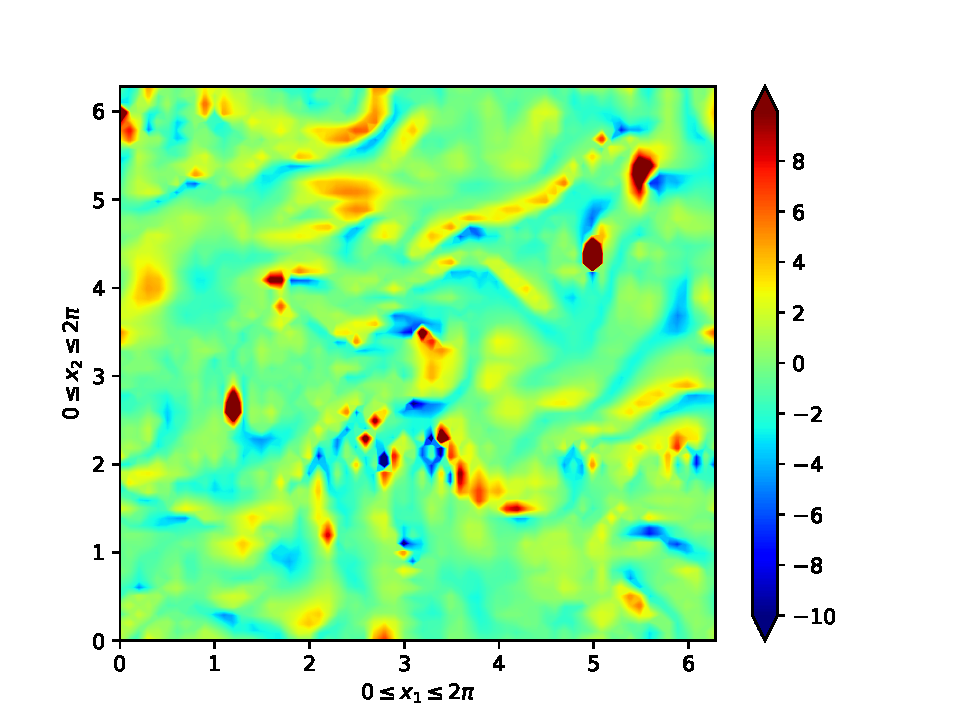
\includegraphics[height=1.75in]{media/run-cds-00/ke-RHS-CDS-00}
        \caption{$\frac{1}{k} \frac{Dk}{Dt}$}
    \end{subfigure}
    ~
    \begin{subfigure}[H]{0.45\textwidth}
        \includegraphics[height=1.75in]{media/run-cds-00/enstrophy-RHS-CDS-00}
        \caption{$\frac{1}{\Omega} \frac{D \Omega}{Dt}$}
    \end{subfigure}
    \newline
    \begin{subfigure}{0.45\textwidth}
        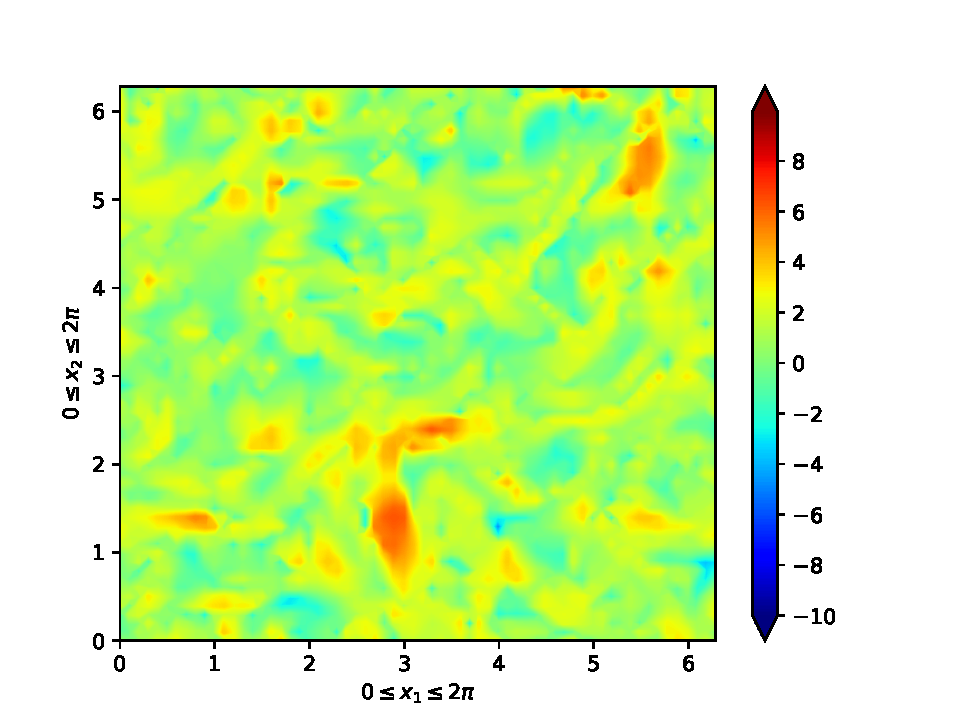
\includegraphics[height=1.75in]{media/run-cds-00/A-enst-CDS-00}
        \caption{$A_{\Omega}$}
    \end{subfigure}
    ~
    \begin{subfigure}{0.45\textwidth}
        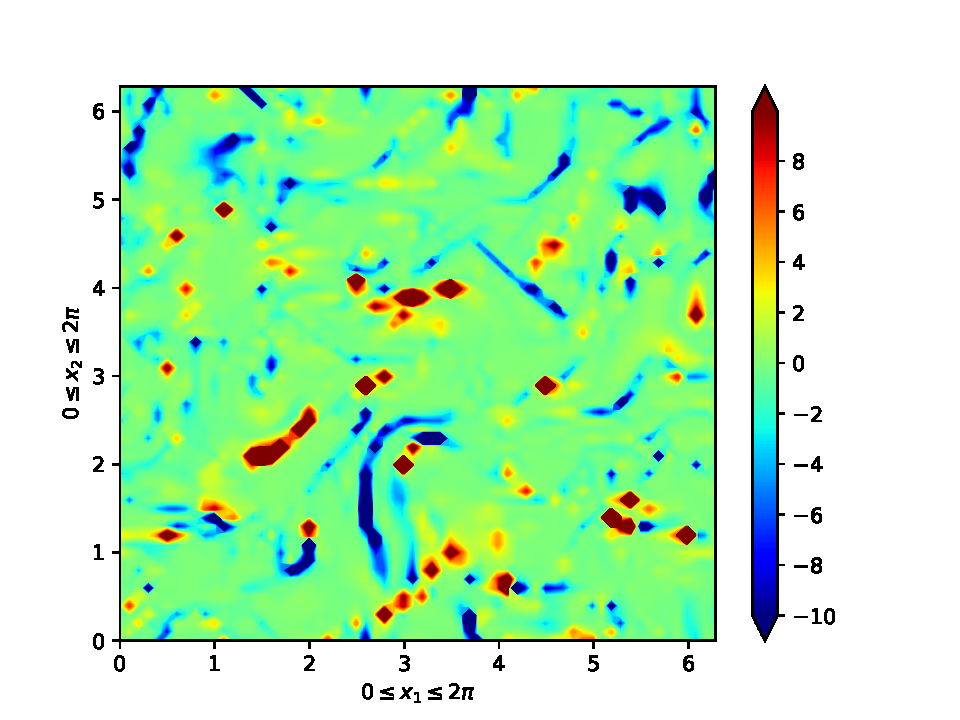
\includegraphics[height=1.75in]{media/run-cds-00/trans-enst-CDS-00}
        \caption{$\Pi_{\Omega}$}
    \end{subfigure}
    \newline
    \begin{subfigure}{0.45\textwidth}
        \includegraphics[height=1.75in]{media/run-cds-00/prod-enst-CDS-00}
        \caption{$P_{\Omega}$}
    \end{subfigure}
    ~
    \begin{subfigure}{0.45\textwidth}
        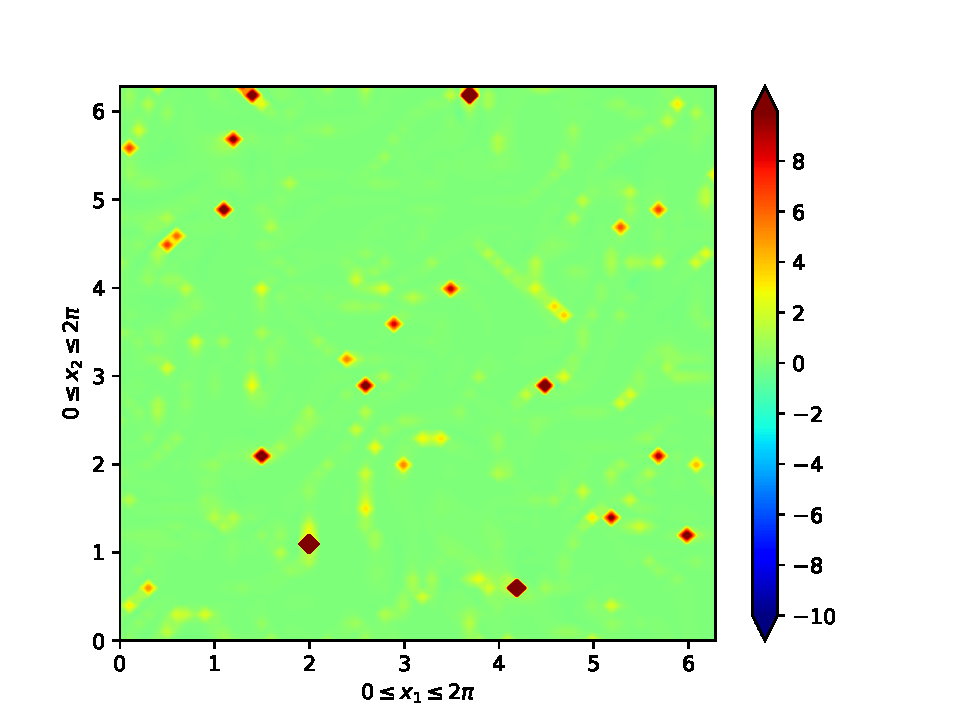
\includegraphics[height=1.75in]{media/run-cds-00/B-enst-CDS-00}
        \caption{$B_{\Omega}$}
    \end{subfigure}
    \newline
    \begin{subfigure}{0.45\textwidth}
        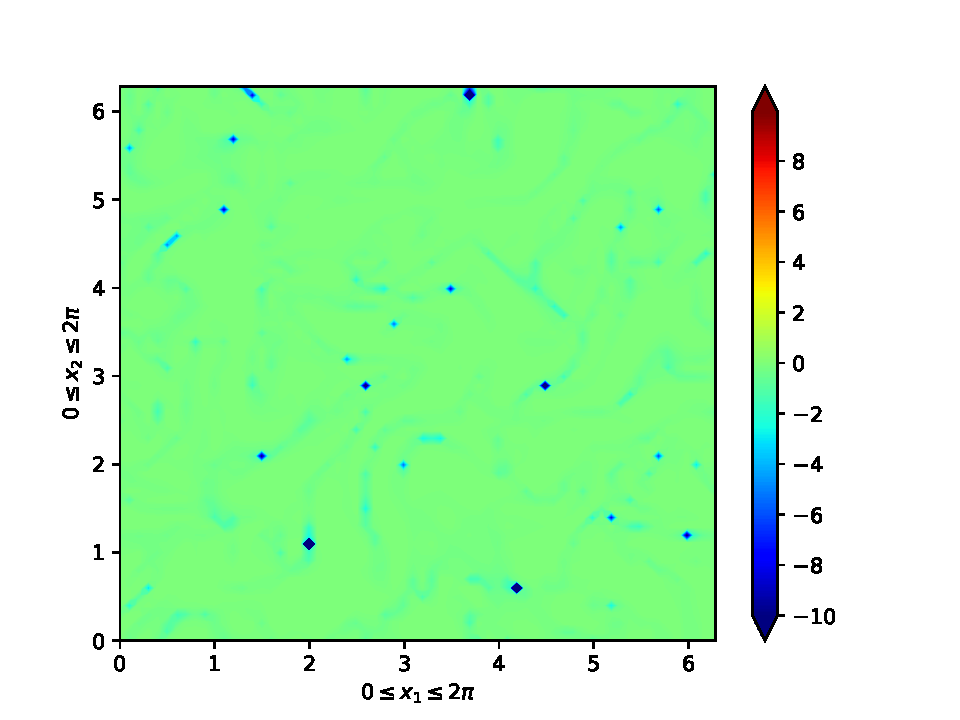
\includegraphics[height=1.75in]{media/run-cds-00/D-enst-CDS-00}
        \caption{$D_{\Omega}$}
    \end{subfigure}
\end{figure}
%\newpage

%------------------------------------------------------------------------------%
% 1330                                                                         %
%------------------------------------------------------------------------------%
%\subsubsection{$t=30.04$ i.e., 1st time step where $C_{DS}=0.65$ is applied} 
\begin{figure}[H]
    \begin{subfigure}[H]{0.45\textwidth}
        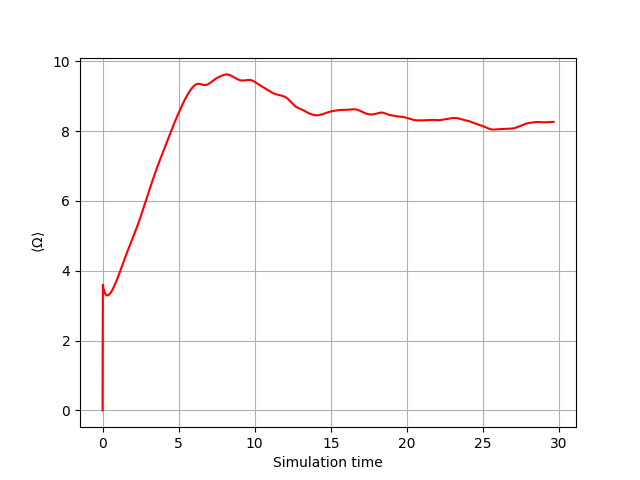
\includegraphics[height=1.75in]{media/run-cds-65/enst-average1330}
        \caption{Average kinetic energy}
    \end{subfigure}
    ~
    \begin{subfigure}[H]{0.45\textwidth}
        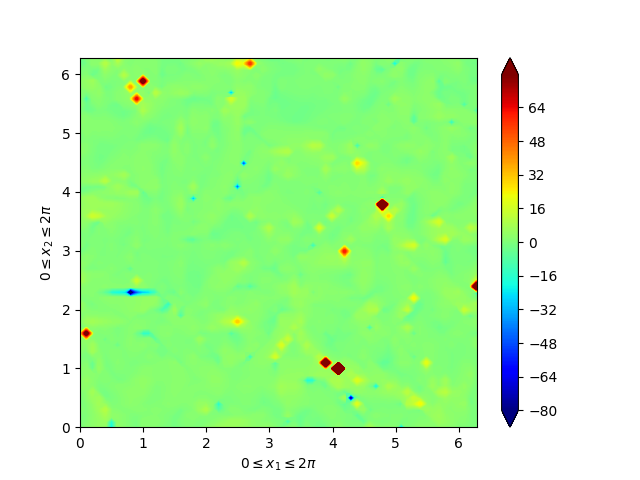
\includegraphics[height=1.75in]{media/run-cds-65/enst-1330}
        \caption{$\frac{1}{\Omega} \frac{D \Omega}{Dt}$}
    \end{subfigure}
    \newline
    \begin{subfigure}{0.45\textwidth}
        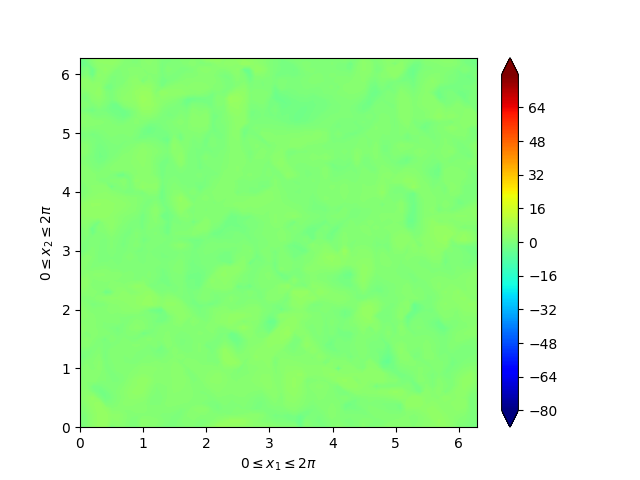
\includegraphics[height=1.75in]{media/run-cds-65/A-enst-1330}
        \caption{$A_{\Omega}$}
    \end{subfigure}
    ~
    \begin{subfigure}{0.45\textwidth}
        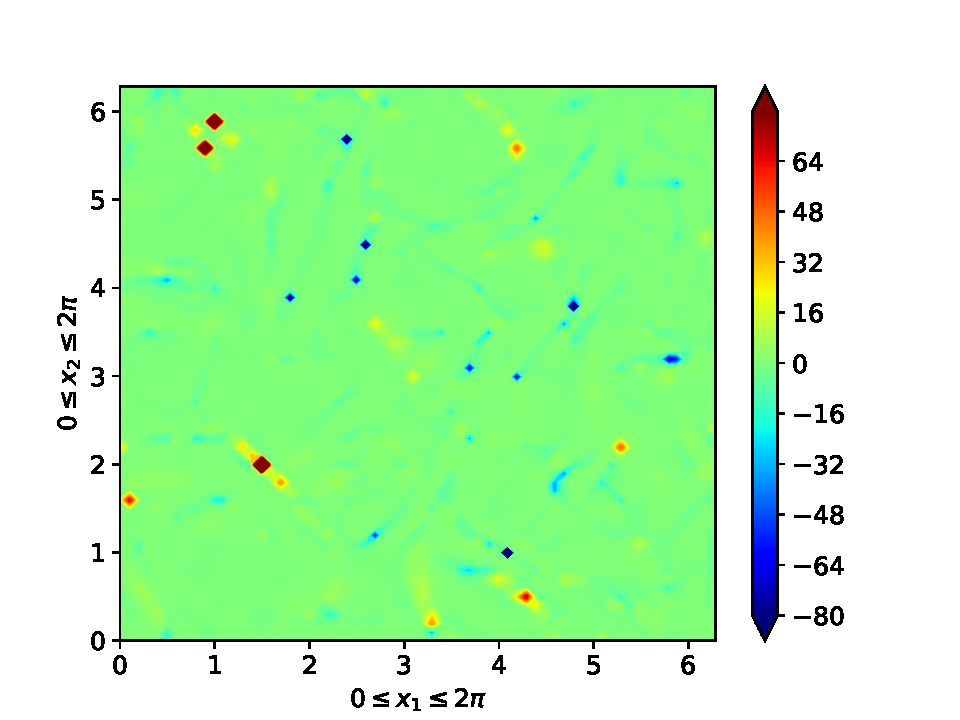
\includegraphics[height=1.75in]{media/run-cds-65/Pi-enst-1330}
        \caption{$\Pi_{\Omega}$}
    \end{subfigure}
    \newline
    \begin{subfigure}{0.45\textwidth}
        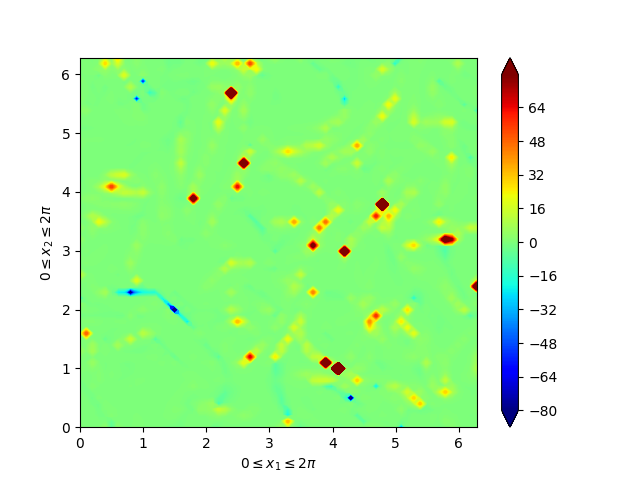
\includegraphics[height=1.75in]{media/run-cds-65/P-enst-1330}
        \caption{$P_{\Omega}$}
    \end{subfigure}
    ~
    \begin{subfigure}{0.45\textwidth}
        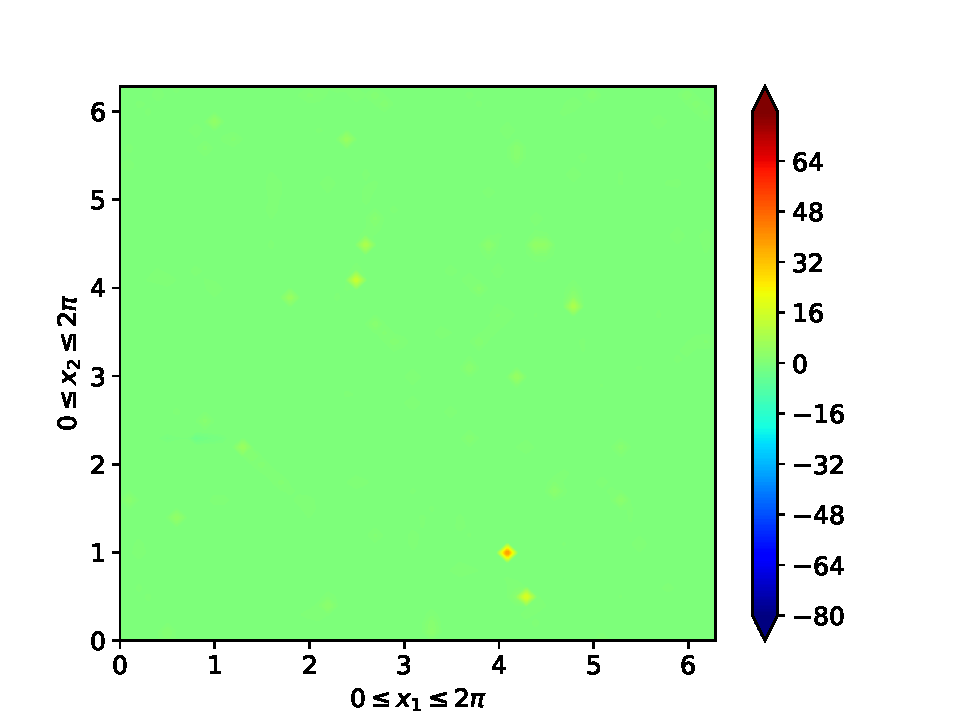
\includegraphics[height=1.75in]{media/run-cds-65/B-enst-1330}
        \caption{$B_{\Omega}$}
    \end{subfigure}
    \newline
    \begin{subfigure}{0.45\textwidth}
        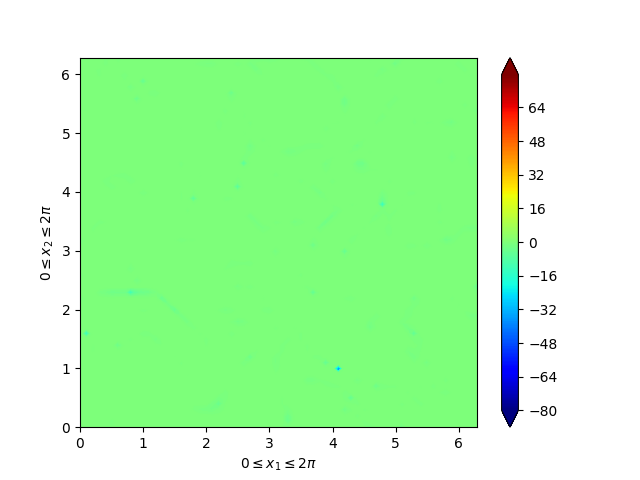
\includegraphics[height=1.75in]{media/run-cds-65/D-enst-1330}
        \caption{$D_{\Omega}$}
    \end{subfigure}
    \caption{Enstrophy transport terms for $t=29.65$, i.e., $t=t^{\ast} - 10 \Delta t$}
\end{figure}

\newpage

\begin{figure}[H]
    \begin{subfigure}[H]{0.45\textwidth}
        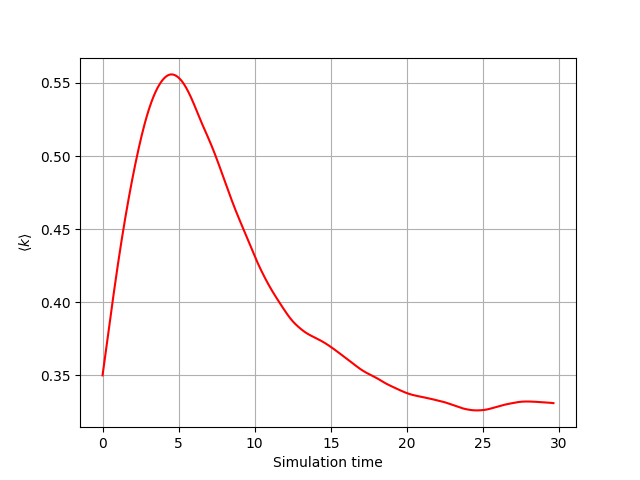
\includegraphics[height=1.75in]{media/run-cds-65/ke-average1330}
        \caption{Average kinetic energy}
    \end{subfigure}
    ~
    \begin{subfigure}[H]{0.45\textwidth}
        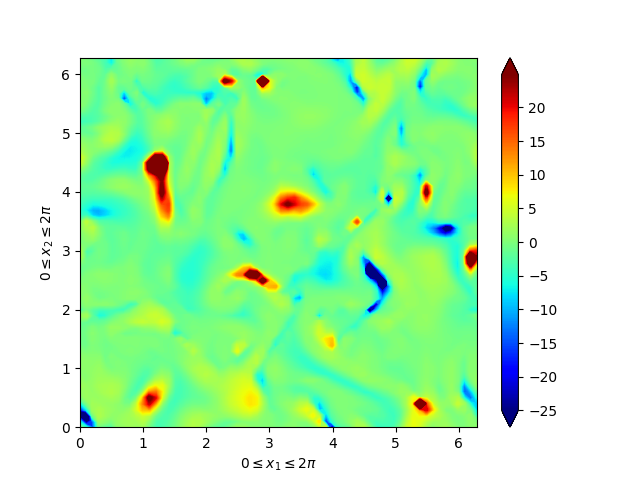
\includegraphics[height=1.75in]{media/run-cds-65/ke-1330}
        \caption{$\frac{1}{k} \frac{D k}{Dt}$}
    \end{subfigure}
    \newline
    \begin{subfigure}{0.45\textwidth}
        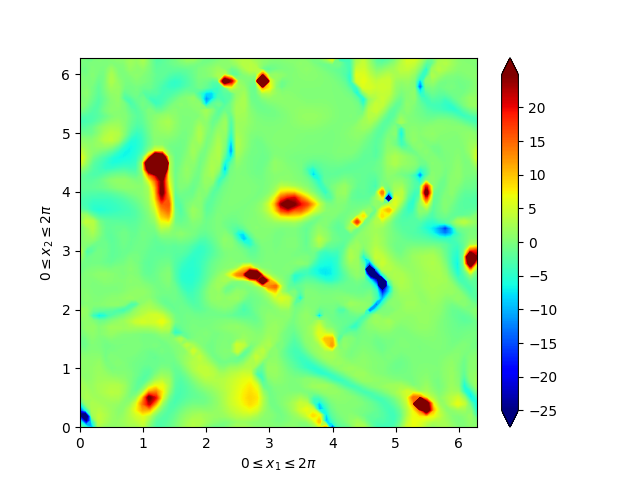
\includegraphics[height=1.75in]{media/run-cds-65/A-ke-1330}
        \caption{$A$}
    \end{subfigure}
    ~
    \begin{subfigure}{0.45\textwidth}
        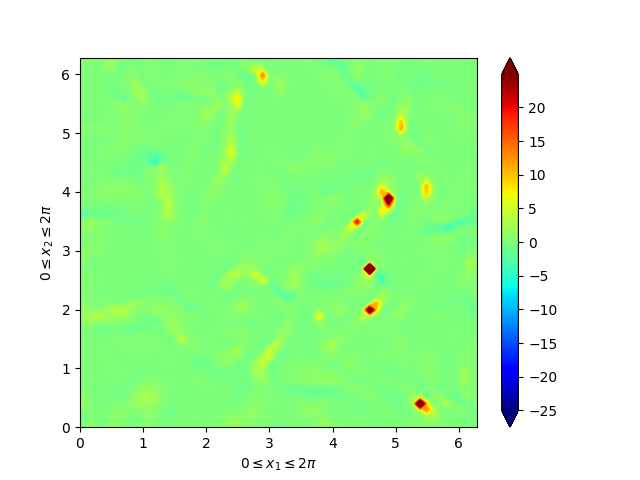
\includegraphics[height=1.75in]{media/run-cds-65/C-ke-1330}
        \caption{$C$}
    \end{subfigure}
    \newline
    \begin{subfigure}{0.45\textwidth}
        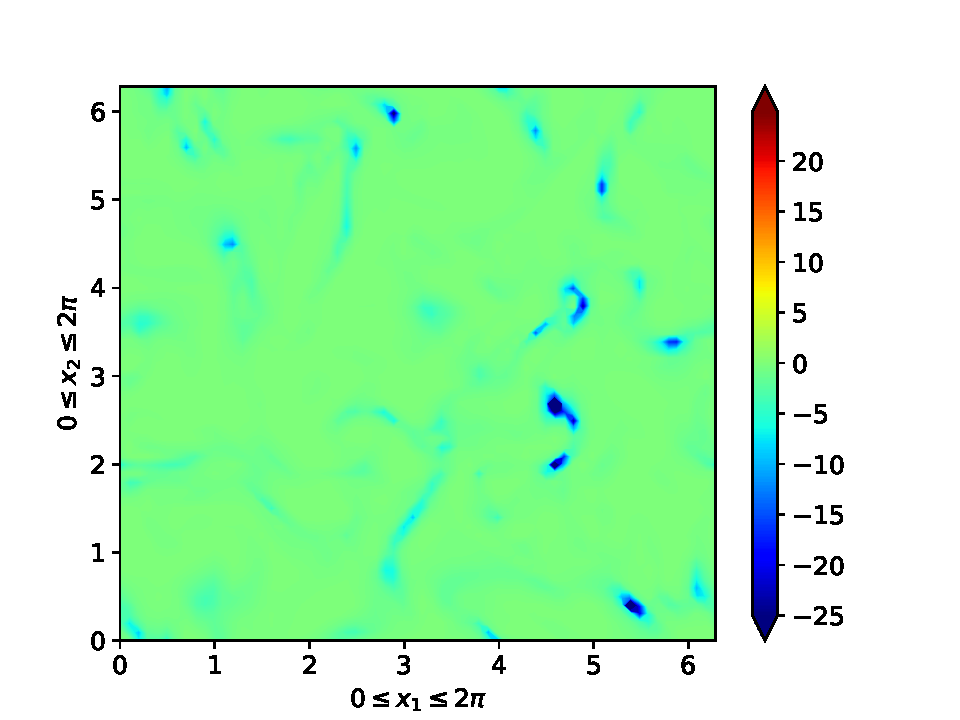
\includegraphics[height=1.75in]{media/run-cds-65/P-ke-1330}
        \caption{$P$}
    \end{subfigure}
    ~
    \begin{subfigure}{0.45\textwidth}
        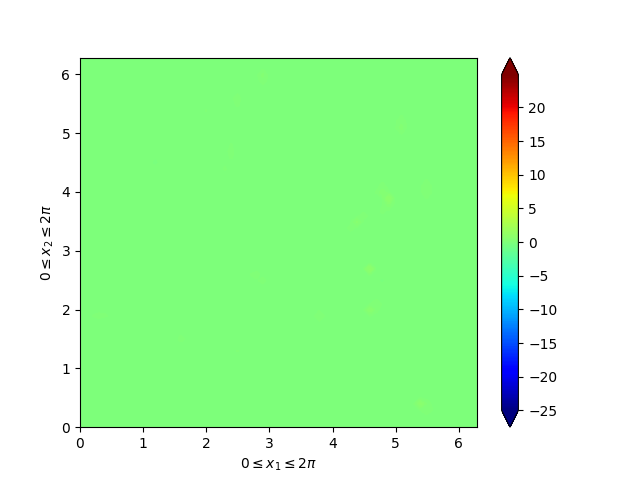
\includegraphics[height=1.75in]{media/run-cds-65/B-ke-1330}
        \caption{$B$}
    \end{subfigure}
    \newline
    \begin{subfigure}{0.45\textwidth}
        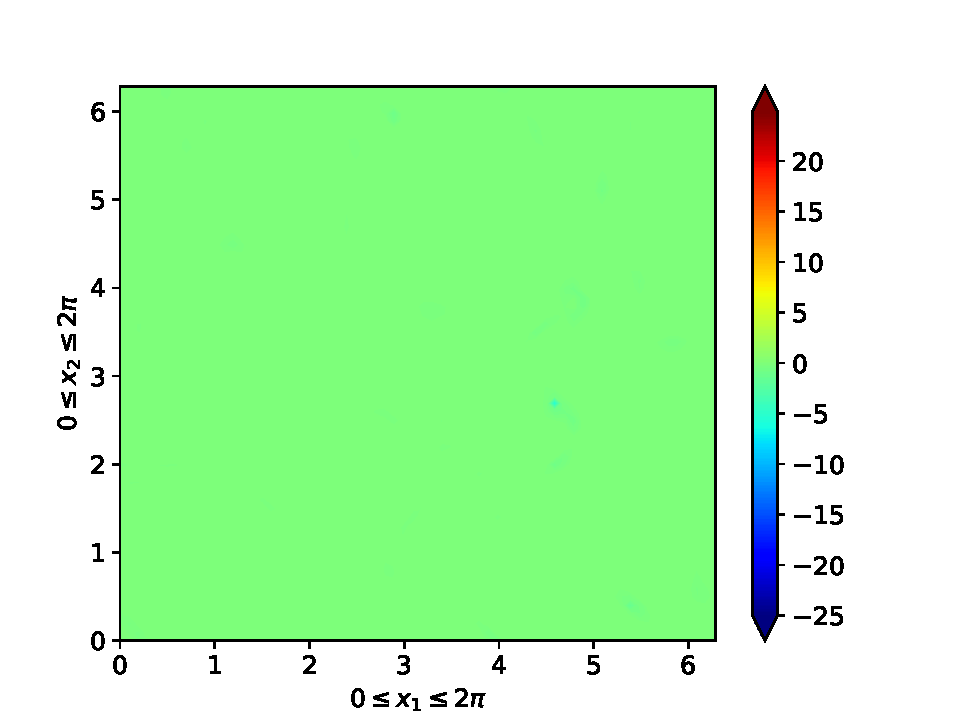
\includegraphics[height=1.75in]{media/run-cds-65/D-ke-1330}
        \caption{$D$}
    \end{subfigure}
    \caption{Kinetic energy transport terms for $t=29.65$, i.e., $t=t^{\ast} - 10 \Delta t$}
\end{figure}

\newpage

%------------------------------------------------------------------------------%
% 1340                                                                         %
%------------------------------------------------------------------------------%
%\subsubsection{$t=30.04$ i.e., 1st time step where $C_{DS}=0.65$ is applied} 
\begin{figure}[H]
    \begin{subfigure}[H]{0.45\textwidth}
        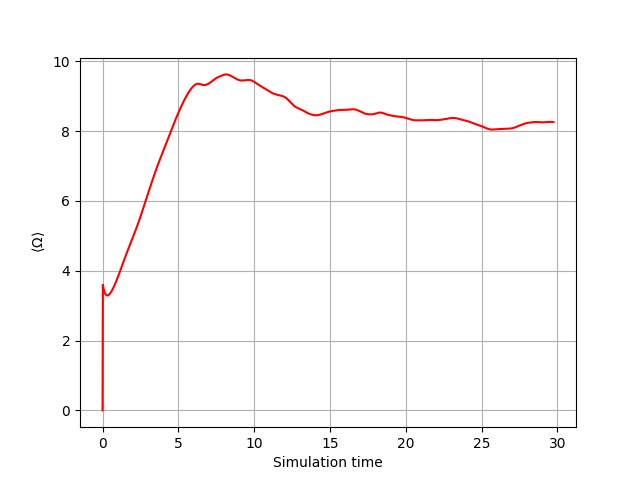
\includegraphics[height=1.75in]{media/run-cds-65/enst-average1335}
        \caption{Average kinetic energy}
    \end{subfigure}
    ~
    \begin{subfigure}[H]{0.45\textwidth}
        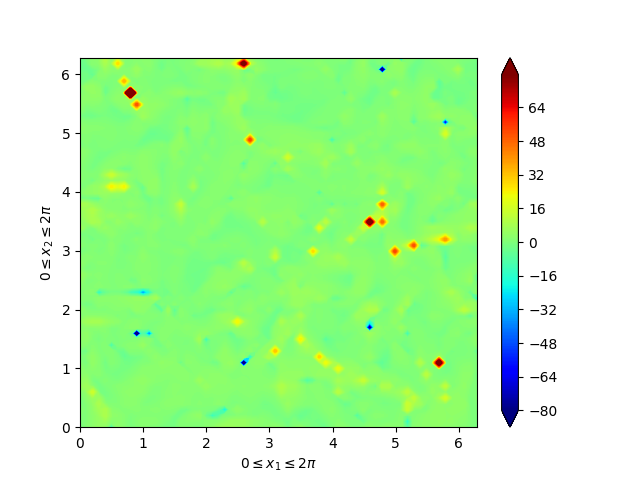
\includegraphics[height=1.75in]{media/run-cds-65/enst-1335}
        \caption{$\frac{1}{\Omega} \frac{D \Omega}{Dt}$}
    \end{subfigure}
    \newline
    \begin{subfigure}{0.45\textwidth}
        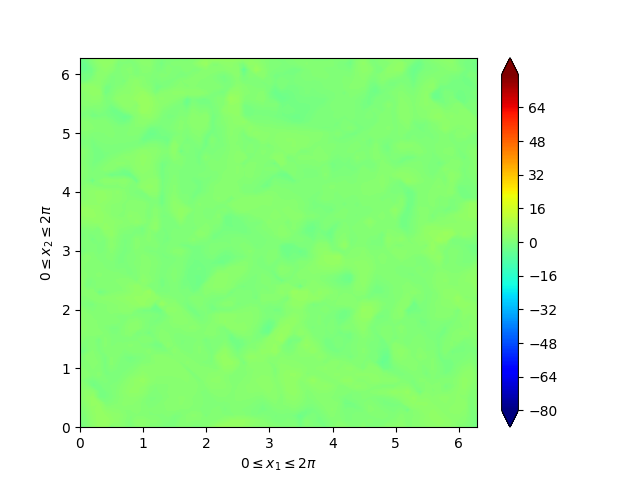
\includegraphics[height=1.75in]{media/run-cds-65/A-enst-1335}
        \caption{$A_{\Omega}$}
    \end{subfigure}
    ~
    \begin{subfigure}{0.45\textwidth}
        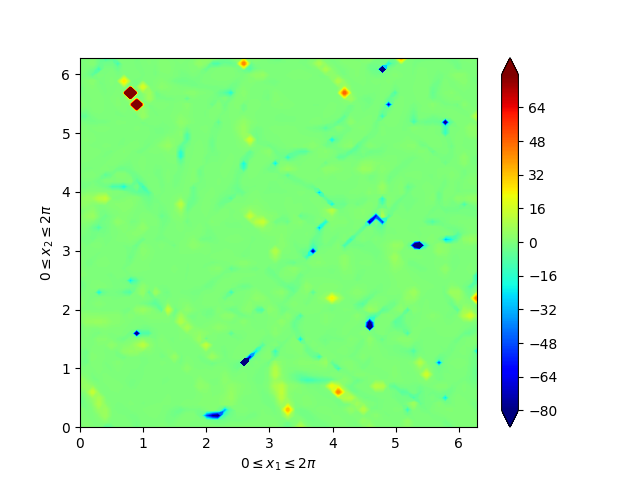
\includegraphics[height=1.75in]{media/run-cds-65/Pi-enst-1335}
        \caption{$\Pi_{\Omega}$}
    \end{subfigure}
    \newline
    \begin{subfigure}{0.45\textwidth}
        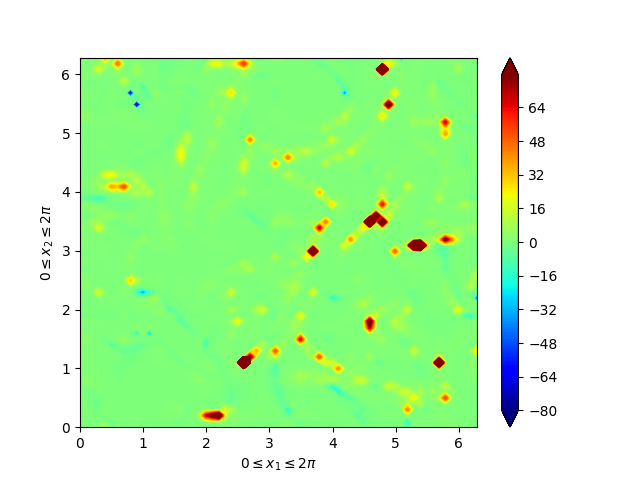
\includegraphics[height=1.75in]{media/run-cds-65/P-enst-1335}
        \caption{$P_{\Omega}$}
    \end{subfigure}
    ~
    \begin{subfigure}{0.45\textwidth}
        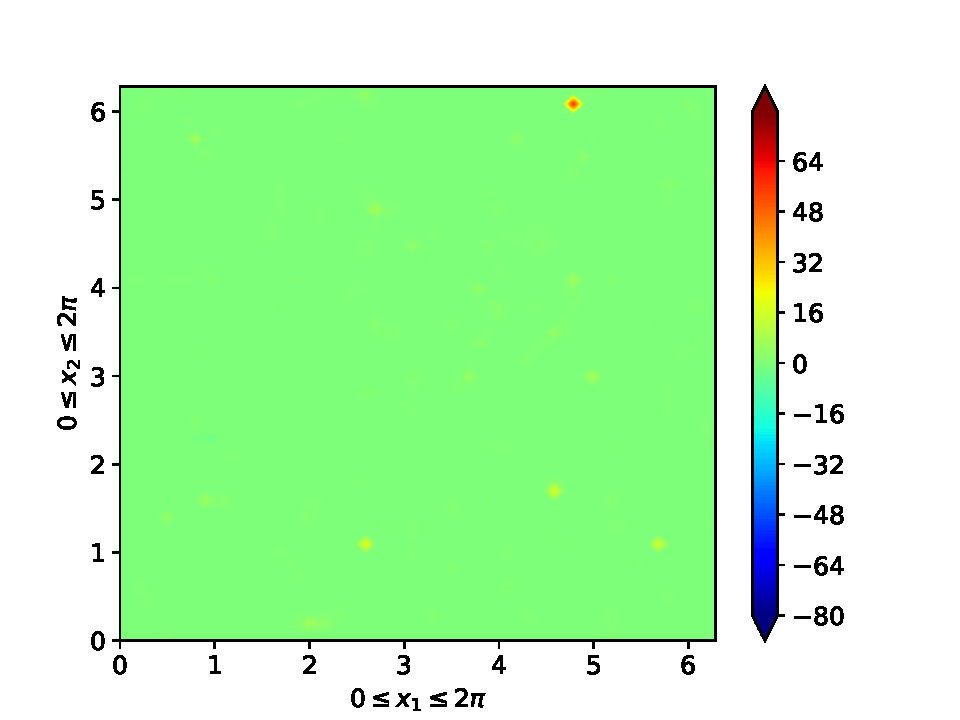
\includegraphics[height=1.75in]{media/run-cds-65/B-enst-1335}
        \caption{$B_{\Omega}$}
    \end{subfigure}
    \newline
    \begin{subfigure}{0.45\textwidth}
        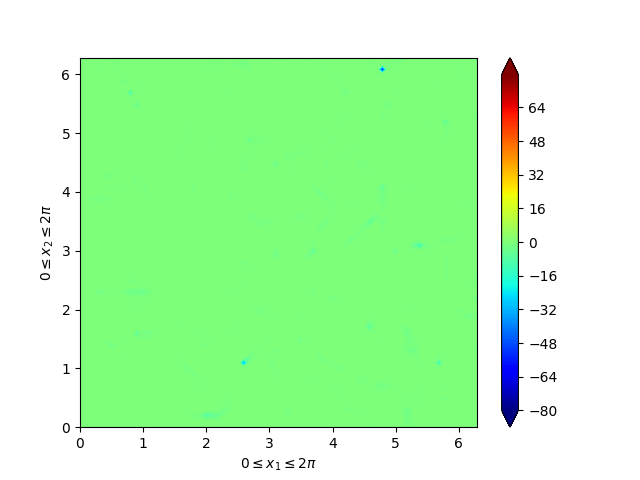
\includegraphics[height=1.75in]{media/run-cds-65/D-enst-1335}
        \caption{$D_{\Omega}$}
    \end{subfigure}
    \caption{Enstrophy transport terms for $t=29.77$, i.e., $t=t^{\ast} - 5 \Delta t$}
\end{figure}

\newpage

\begin{figure}[H]
    \begin{subfigure}[H]{0.45\textwidth}
        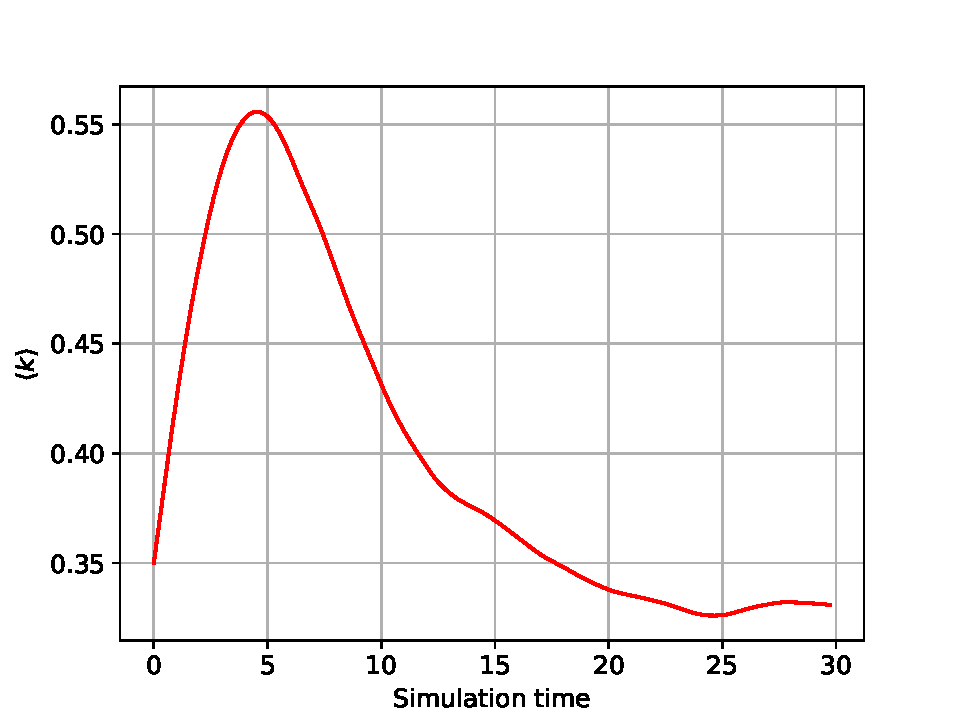
\includegraphics[height=1.75in]{media/run-cds-65/ke-average1335}
        \caption{Average kinetic energy}
    \end{subfigure}
    ~
    \begin{subfigure}[H]{0.45\textwidth}
        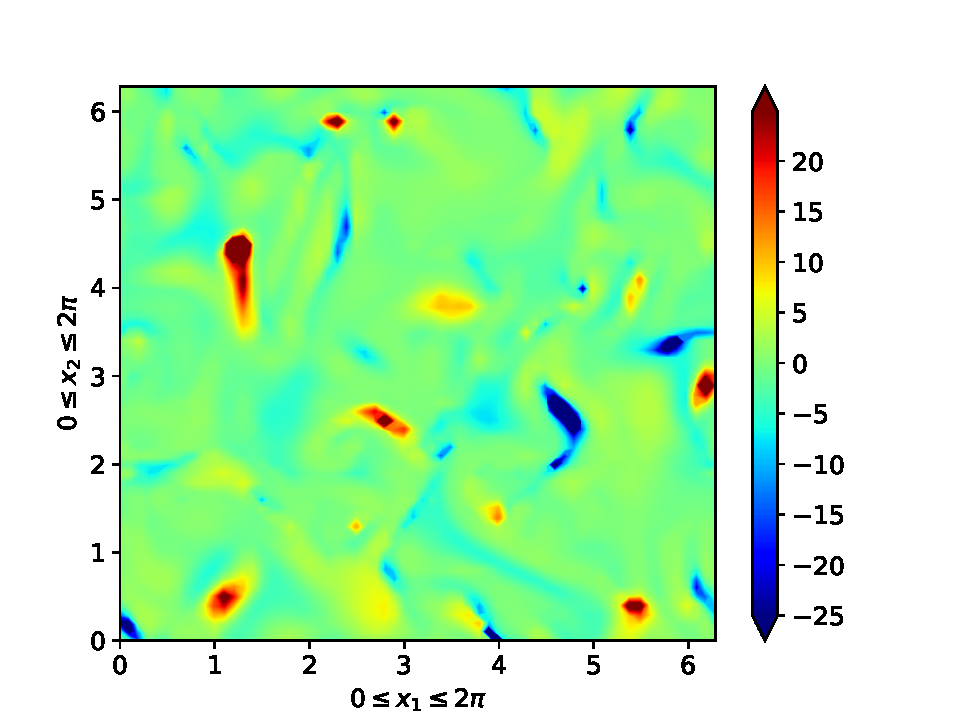
\includegraphics[height=1.75in]{media/run-cds-65/ke-1335}
        \caption{$\frac{1}{k} \frac{D k}{Dt}$}
    \end{subfigure}
    \newline
    \begin{subfigure}{0.45\textwidth}
        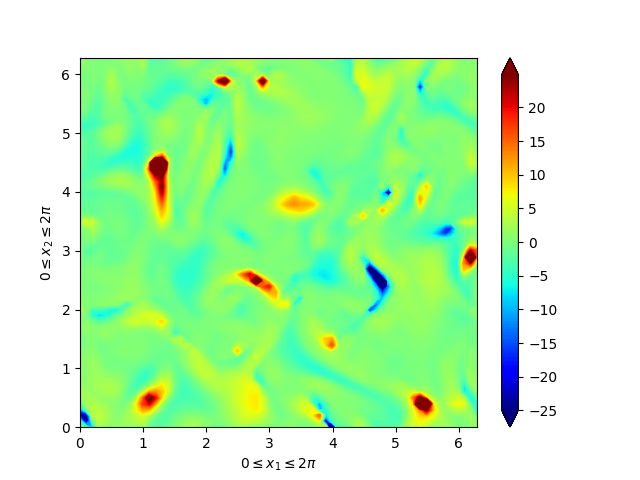
\includegraphics[height=1.75in]{media/run-cds-65/A-ke-1335}
        \caption{$A$}
    \end{subfigure}
    ~
    \begin{subfigure}{0.45\textwidth}
        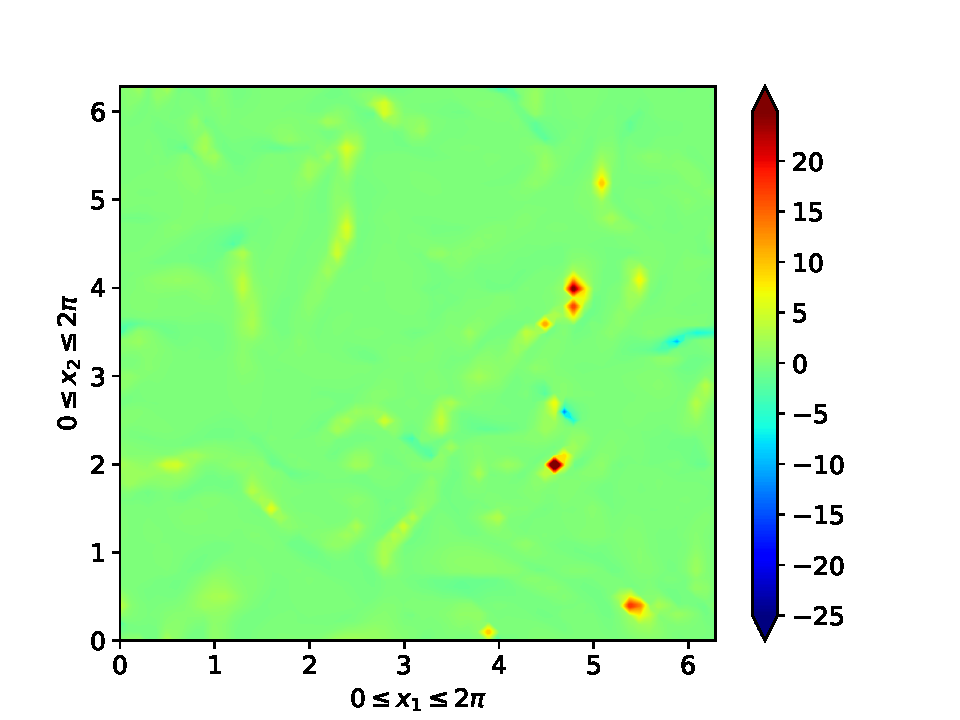
\includegraphics[height=1.75in]{media/run-cds-65/C-ke-1335}
        \caption{$C$}
    \end{subfigure}
    \newline
    \begin{subfigure}{0.45\textwidth}
        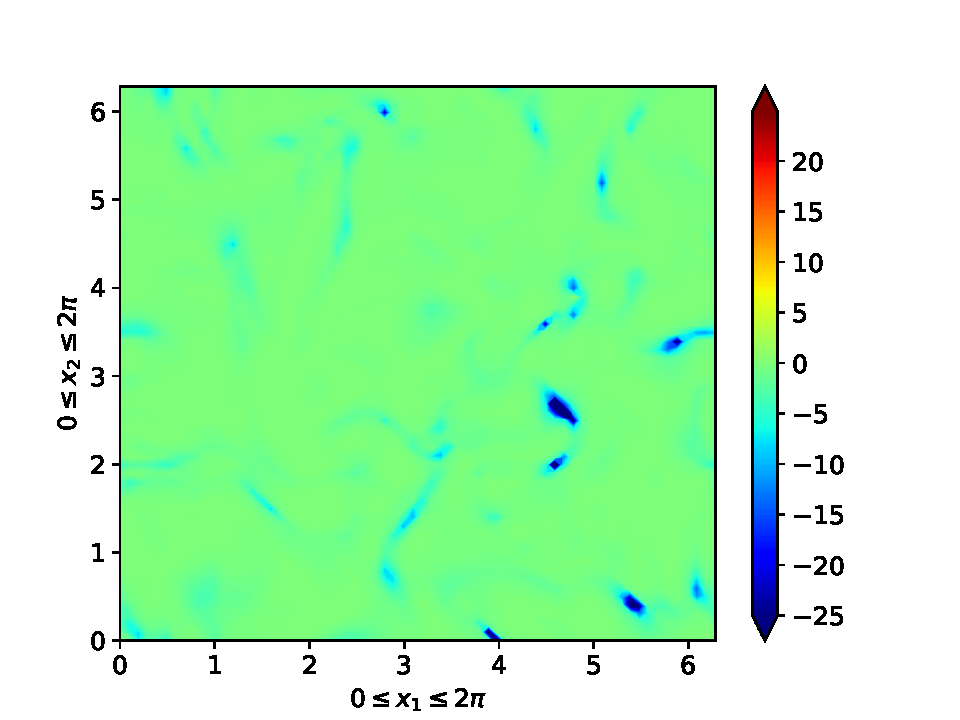
\includegraphics[height=1.75in]{media/run-cds-65/P-ke-1335}
        \caption{$P$}
    \end{subfigure}
    ~
    \begin{subfigure}{0.45\textwidth}
        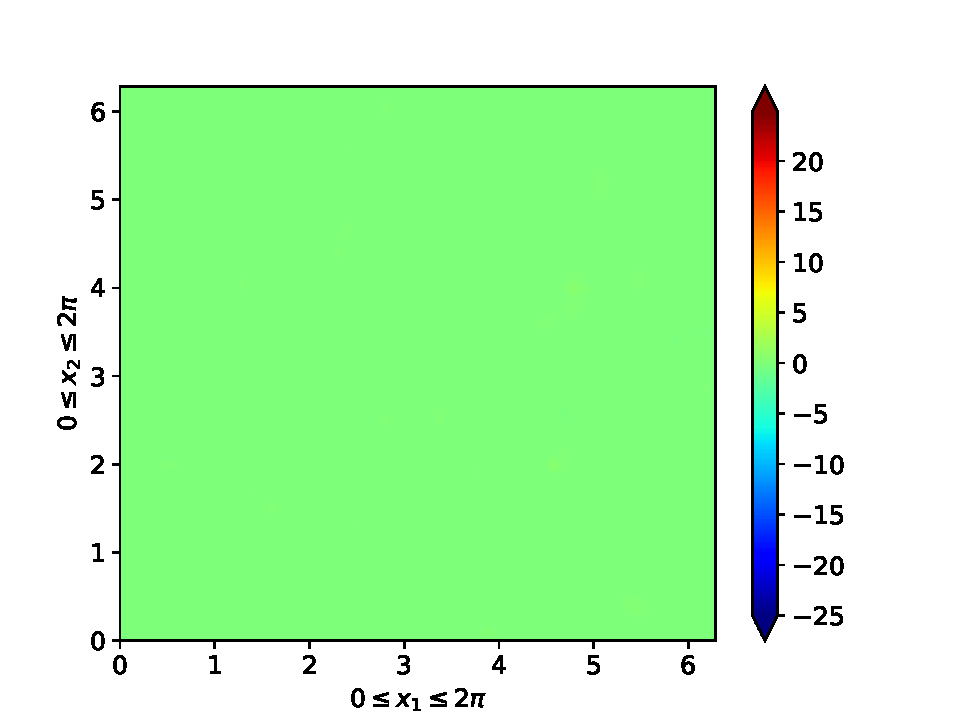
\includegraphics[height=1.75in]{media/run-cds-65/B-ke-1335}
        \caption{$B$}
    \end{subfigure}
    \newline
    \begin{subfigure}{0.45\textwidth}
        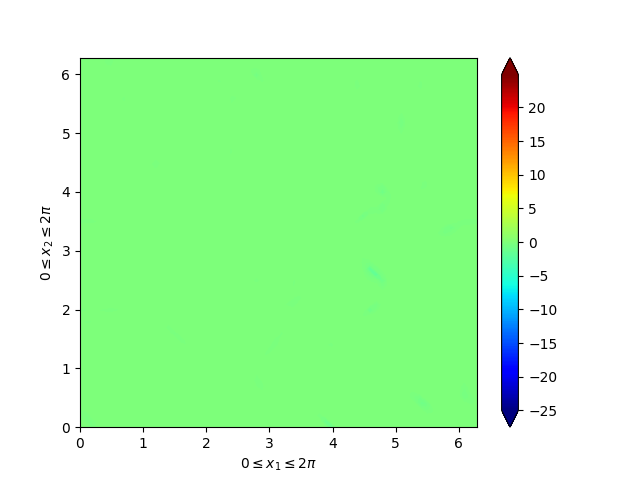
\includegraphics[height=1.75in]{media/run-cds-65/D-ke-1335}
        \caption{$D$}
    \end{subfigure}
    \caption{Kinetic energy transport terms for $t=29.77$, i.e., $t=t^{\ast} - 5 \Delta t$}
\end{figure}

\newpage

%------------------------------------------------------------------------------%
% 1340                                                                         %
%------------------------------------------------------------------------------%
%\subsubsection{$t=30.04$ i.e., 1st time step where $C_{DS}=0.65$ is applied} 
\begin{figure}[H]
    \begin{subfigure}[H]{0.45\textwidth}
        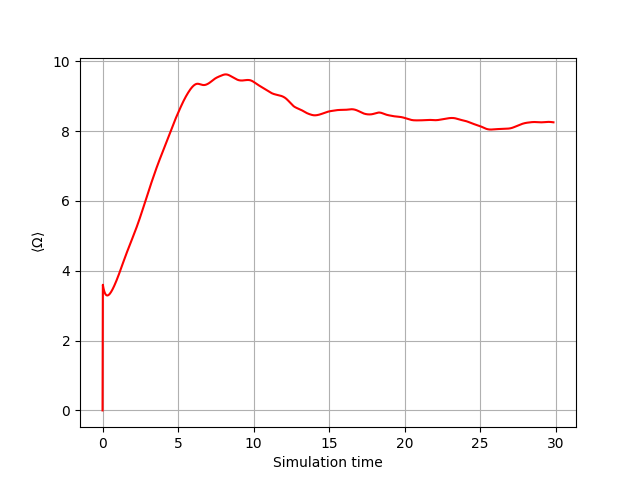
\includegraphics[height=1.75in]{media/run-cds-65/enst-average1340}
        \caption{Average kinetic energy}
    \end{subfigure}
    ~
    \begin{subfigure}[H]{0.45\textwidth}
        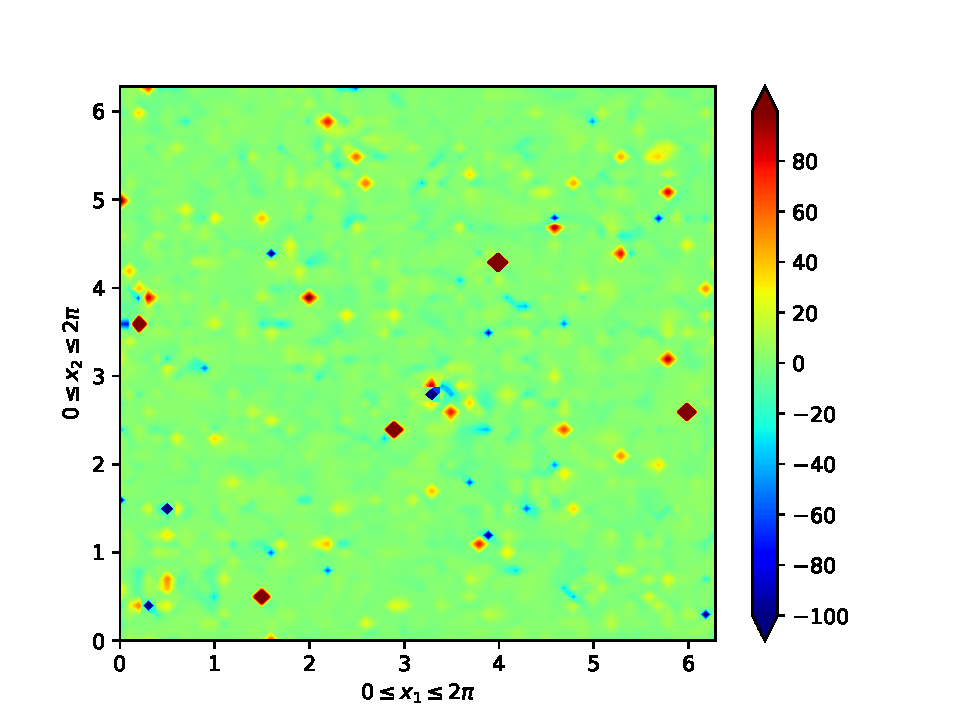
\includegraphics[height=1.75in]{media/run-cds-65/enst-1340}
        \caption{$\frac{1}{\Omega} \frac{D \Omega}{Dt}$}
    \end{subfigure}
    \newline
    \begin{subfigure}{0.45\textwidth}
        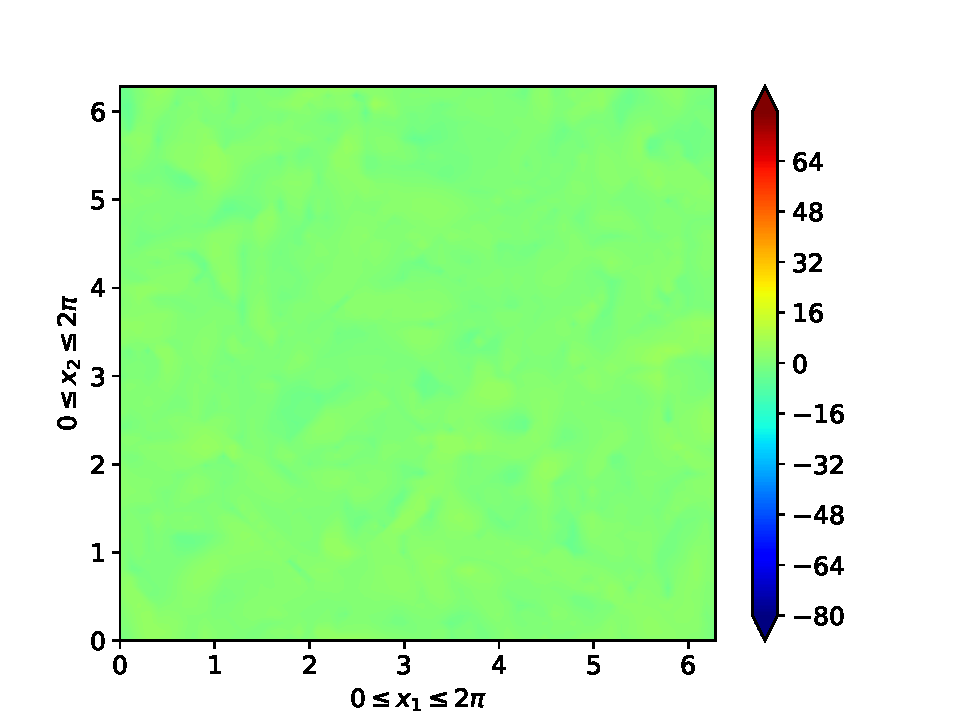
\includegraphics[height=1.75in]{media/run-cds-65/A-enst-1340}
        \caption{$A_{\Omega}$}
    \end{subfigure}
    ~
    \begin{subfigure}{0.45\textwidth}
        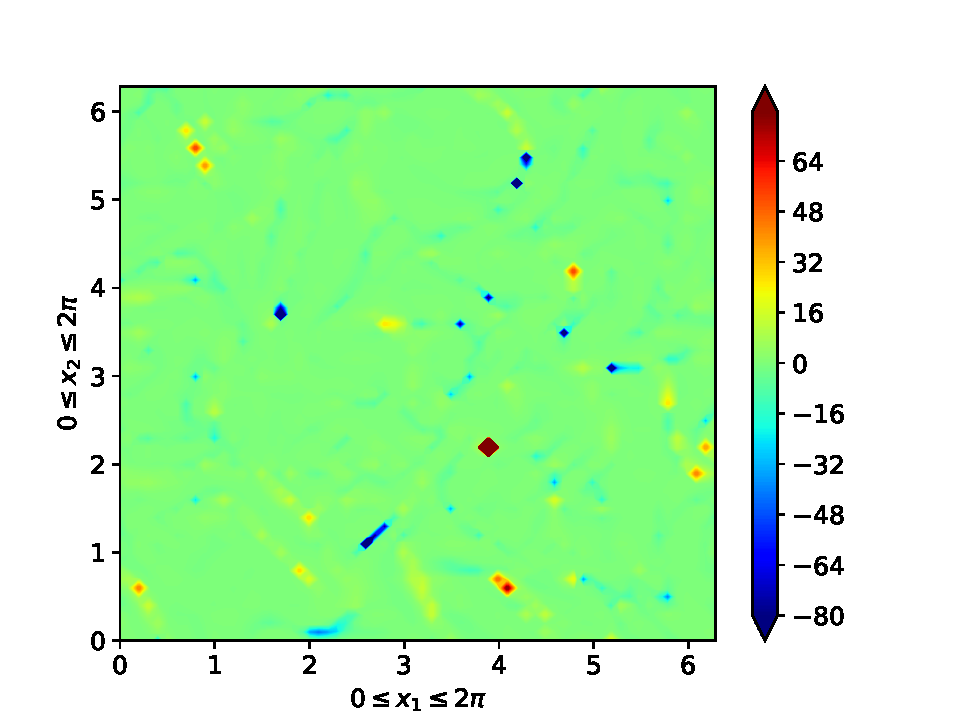
\includegraphics[height=1.75in]{media/run-cds-65/Pi-enst-1340}
        \caption{$\Pi_{\Omega}$}
    \end{subfigure}
    \newline
    \begin{subfigure}{0.45\textwidth}
        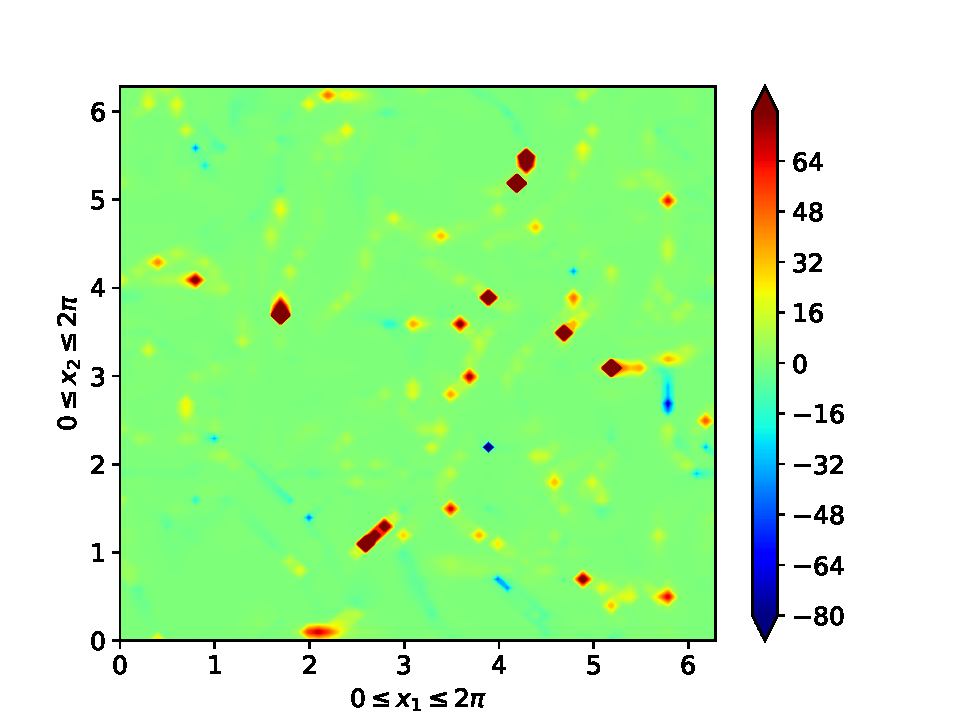
\includegraphics[height=1.75in]{media/run-cds-65/P-enst-1340}
        \caption{$P_{\Omega}$}
    \end{subfigure}
    ~
    \begin{subfigure}{0.45\textwidth}
        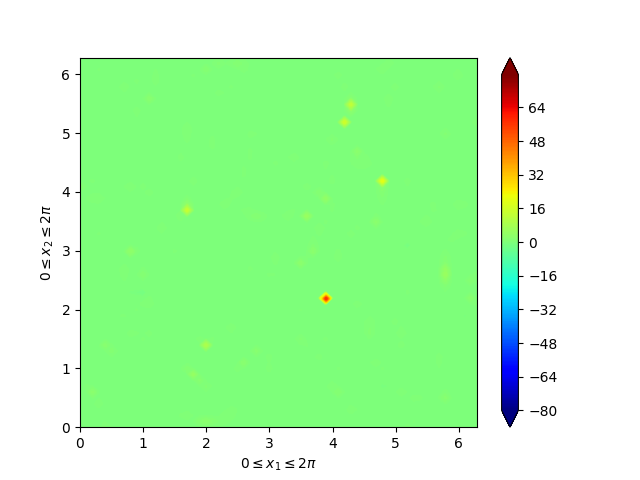
\includegraphics[height=1.75in]{media/run-cds-65/B-enst-1340}
        \caption{$B_{\Omega}$}
    \end{subfigure}
    \newline
    \begin{subfigure}{0.45\textwidth}
        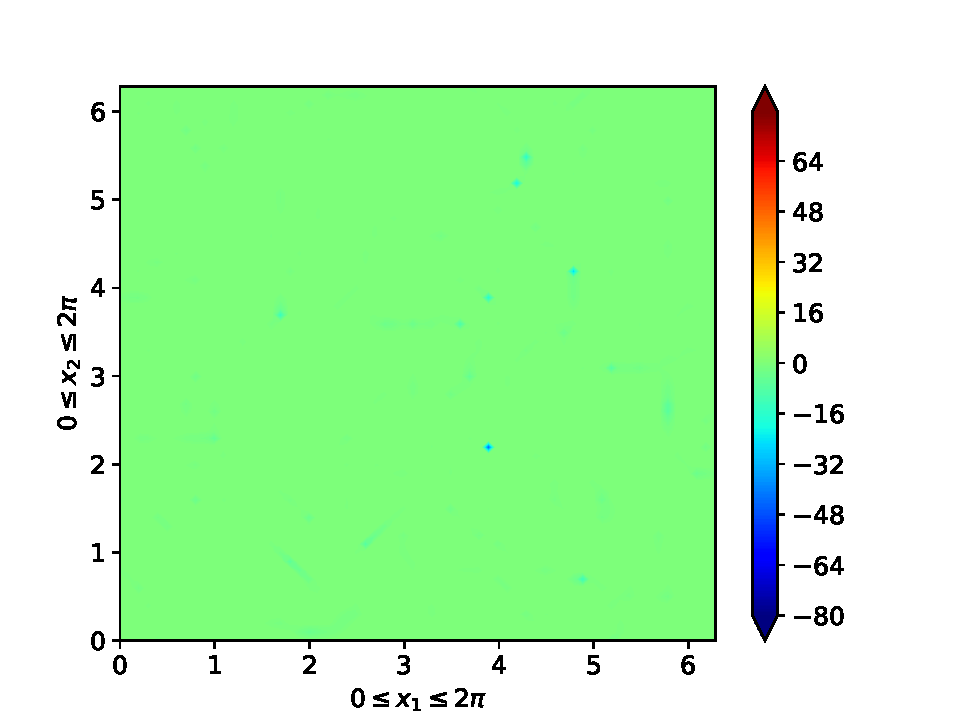
\includegraphics[height=1.75in]{media/run-cds-65/D-enst-1340}
        \caption{$D_{\Omega}$}
    \end{subfigure}
    \caption{Enstrophy transport terms for $t=29.88$, i.e., $t=t^{\ast} $}
\end{figure}

\newpage

\begin{figure}[H]
    \begin{subfigure}[H]{0.45\textwidth}
        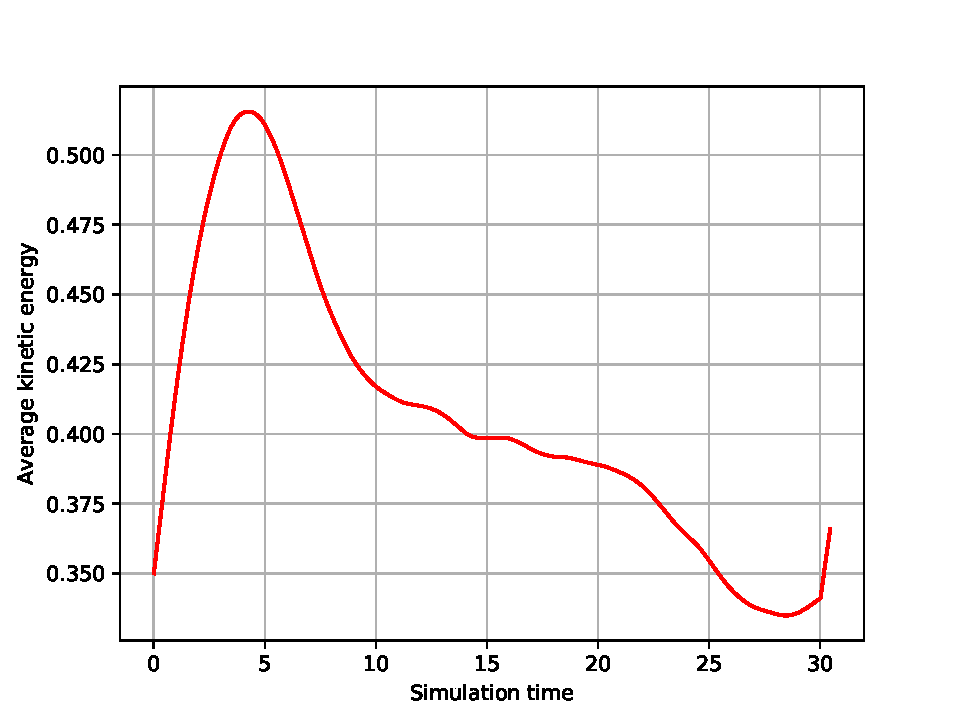
\includegraphics[height=1.75in]{media/run-cds-65/ke-average1340}
        \caption{Average kinetic energy}
    \end{subfigure}
    ~
    \begin{subfigure}[H]{0.45\textwidth}
        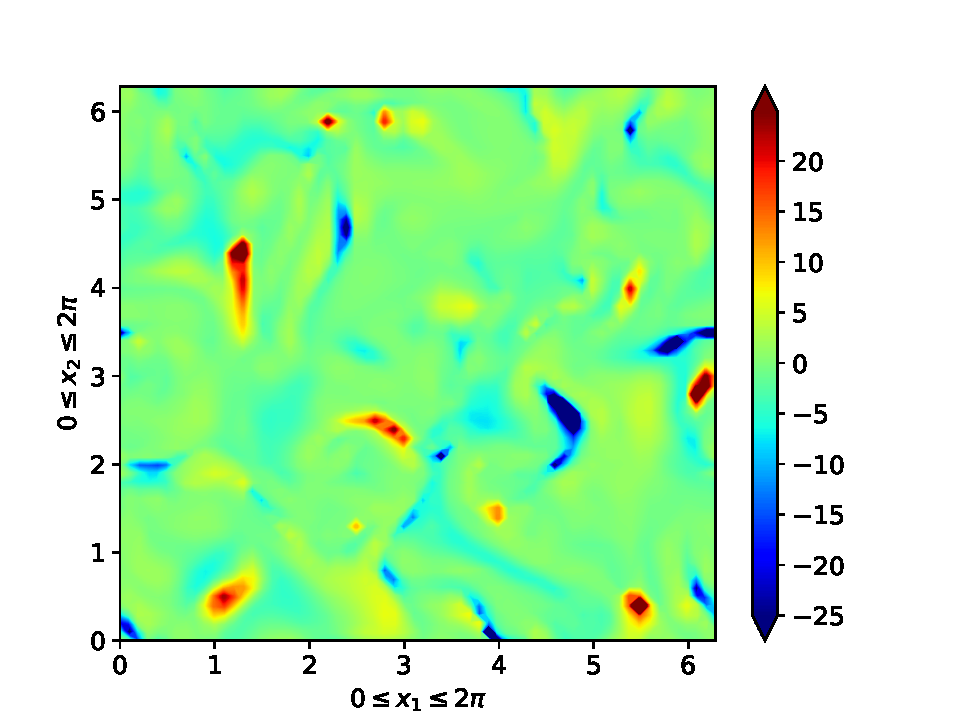
\includegraphics[height=1.75in]{media/run-cds-65/ke-1340}
        \caption{$\frac{1}{k} \frac{D k}{Dt}$}
    \end{subfigure}
    \newline
    \begin{subfigure}{0.45\textwidth}
        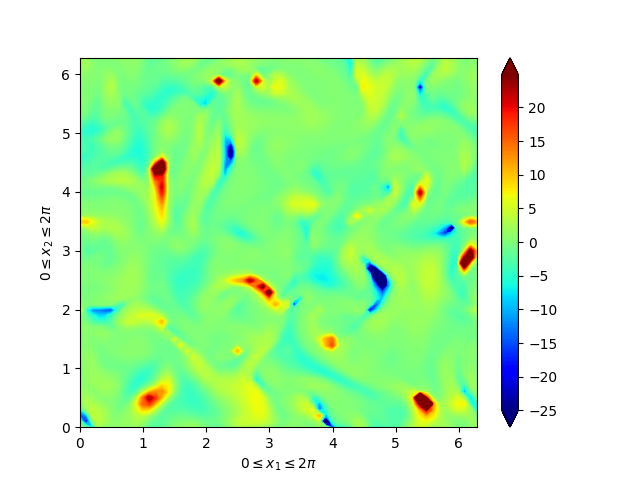
\includegraphics[height=1.75in]{media/run-cds-65/A-ke-1340}
        \caption{$A$}
    \end{subfigure}
    ~
    \begin{subfigure}{0.45\textwidth}
        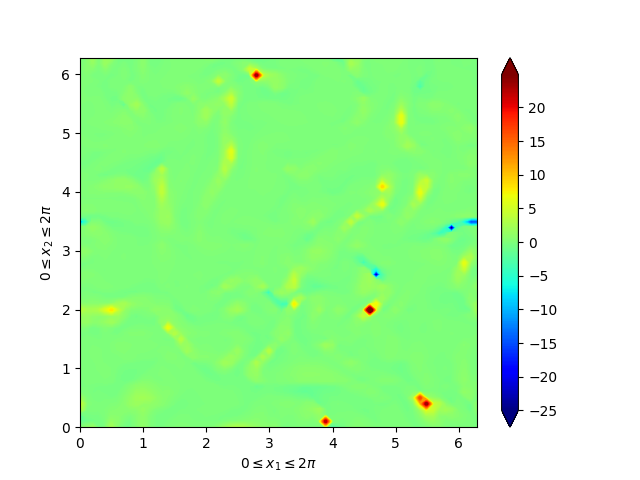
\includegraphics[height=1.75in]{media/run-cds-65/C-ke-1340}
        \caption{$C$}
    \end{subfigure}
    \newline
    \begin{subfigure}{0.45\textwidth}
        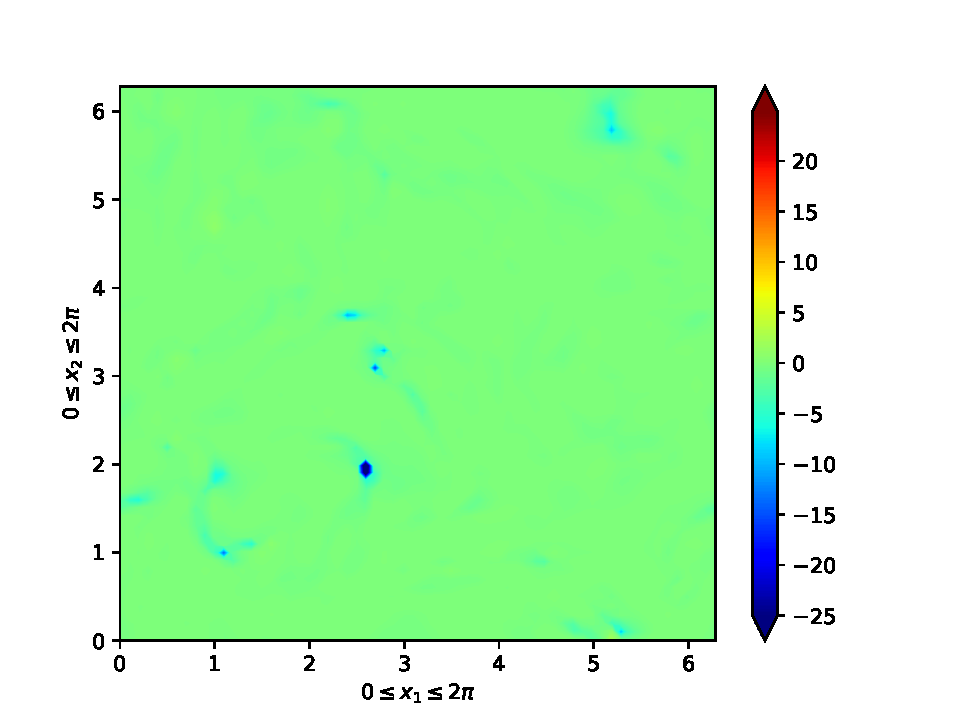
\includegraphics[height=1.75in]{media/run-cds-65/P-ke-1340}
        \caption{$P$}
    \end{subfigure}
    ~
    \begin{subfigure}{0.45\textwidth}
        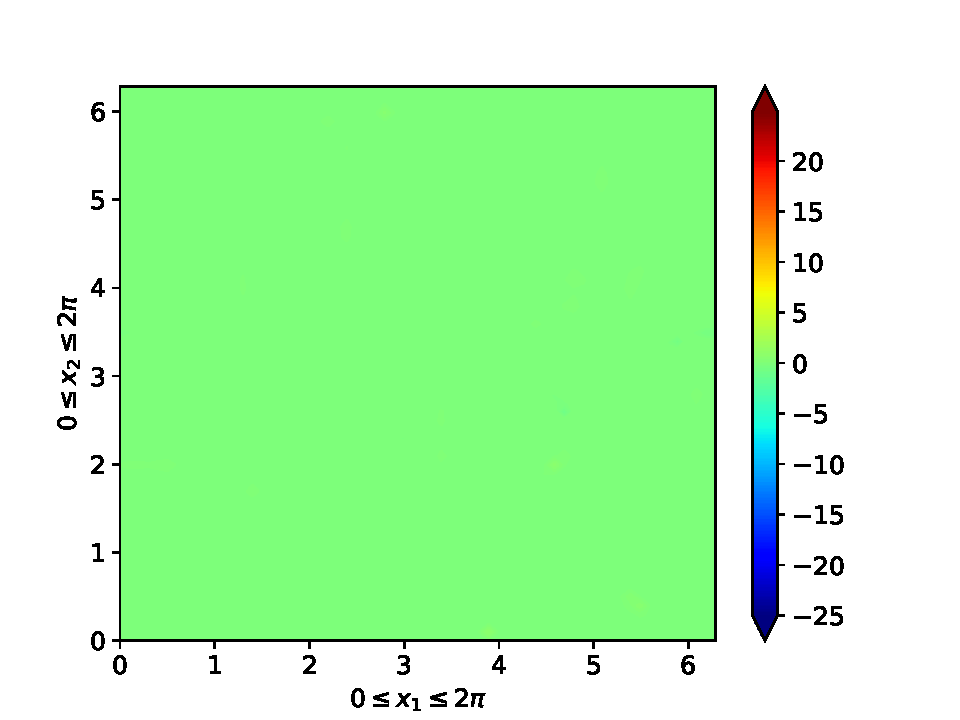
\includegraphics[height=1.75in]{media/run-cds-65/B-ke-1340}
        \caption{$B$}
    \end{subfigure}
    \newline
    \begin{subfigure}{0.45\textwidth}
        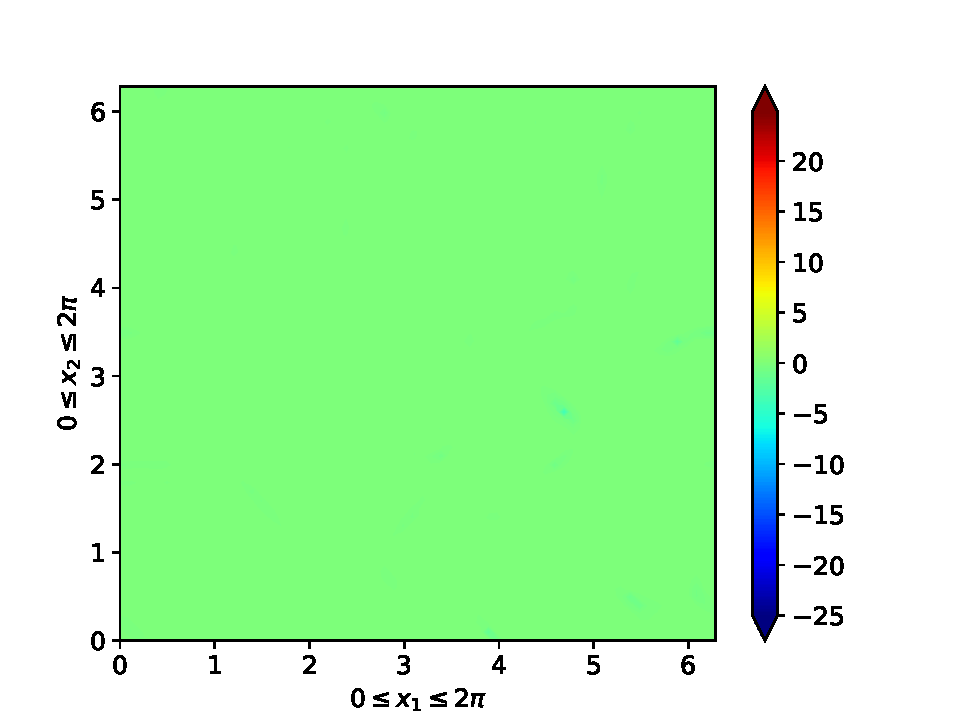
\includegraphics[height=1.75in]{media/run-cds-65/D-ke-1340}
        \caption{$D$}
    \end{subfigure}
    \caption{Kinetic energy transport terms for $t=29.88$, i.e., $t=t^{\ast} $}
\end{figure}

\newpage

%------------------------------------------------------------------------------%
% 1360                                                                         %
%------------------------------------------------------------------------------%
%\subsubsection{$t=30.04$ i.e., 1st time step where $C_{DS}=0.65$ is applied} 
\begin{figure}[H]
    \begin{subfigure}[H]{0.45\textwidth}
        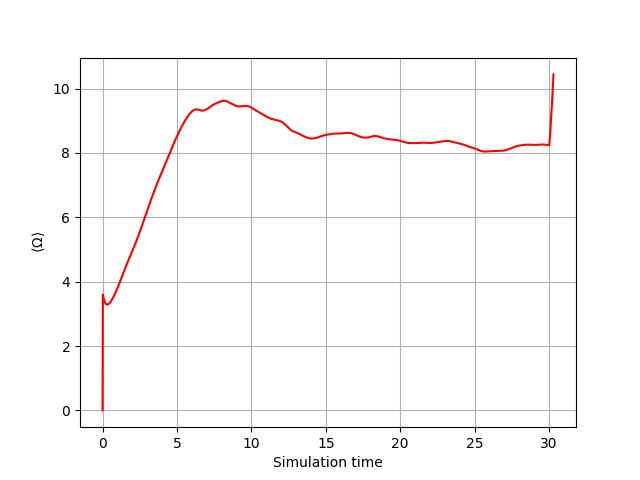
\includegraphics[height=1.75in]{media/run-cds-65/enst-average1360}
        \caption{Average kinetic energy}
    \end{subfigure}
    ~
    \begin{subfigure}[H]{0.45\textwidth}
        \includegraphics[height=1.75in]{media/run-cds-65/enst-1360}
        \caption{$\frac{1}{\Omega} \frac{D \Omega}{Dt}$}
    \end{subfigure}
    \newline
    \begin{subfigure}{0.45\textwidth}
        \includegraphics[height=1.75in]{media/run-cds-65/A-enst-1360}
        \caption{$A_{\Omega}$}
    \end{subfigure}
    ~
    \begin{subfigure}{0.45\textwidth}
        \includegraphics[height=1.75in]{media/run-cds-65/Pi-enst-1360}
        \caption{$\Pi_{\Omega}$}
    \end{subfigure}
    \newline
    \begin{subfigure}{0.45\textwidth}
        \includegraphics[height=1.75in]{media/run-cds-65/P-enst-1360}
        \caption{$P_{\Omega}$}
    \end{subfigure}
    ~
    \begin{subfigure}{0.45\textwidth}
        \includegraphics[height=1.75in]{media/run-cds-65/B-enst-1360}
        \caption{$B_{\Omega}$}
    \end{subfigure}
    \newline
    \begin{subfigure}{0.45\textwidth}
        \includegraphics[height=1.75in]{media/run-cds-65/D-enst-1360}
        \caption{$D_{\Omega}$}
    \end{subfigure}
    \caption{Enstrophy transport terms for $t=30.32$, i.e., $t=t^{\ast} + 20 \Delta t$}
\end{figure}

\newpage

\begin{figure}[H]
    \begin{subfigure}[H]{0.45\textwidth}
        \includegraphics[height=1.75in]{media/run-cds-65/ke-average1360}
        \caption{Average kinetic energy}
    \end{subfigure}
    ~
    \begin{subfigure}[H]{0.45\textwidth}
        \includegraphics[height=1.75in]{media/run-cds-65/ke-1360}
        \caption{$\frac{1}{k} \frac{D k}{Dt}$}
    \end{subfigure}
    \newline
    \begin{subfigure}{0.45\textwidth}
        \includegraphics[height=1.75in]{media/run-cds-65/A-ke-1360}
        \caption{$A$}
    \end{subfigure}
    ~
    \begin{subfigure}{0.45\textwidth}
        \includegraphics[height=1.75in]{media/run-cds-65/C-ke-1360}
        \caption{$C$}
    \end{subfigure}
    \newline
    \begin{subfigure}{0.45\textwidth}
        \includegraphics[height=1.75in]{media/run-cds-65/P-ke-1360}
        \caption{$P$}
    \end{subfigure}
    ~
    \begin{subfigure}{0.45\textwidth}
        \includegraphics[height=1.75in]{media/run-cds-65/B-ke-1360}
        \caption{$B$}
    \end{subfigure}
    \newline
    \begin{subfigure}{0.45\textwidth}
        \includegraphics[height=1.75in]{media/run-cds-65/D-ke-1360}
        \caption{$D$}
    \end{subfigure}
    \caption{Kinetic energy transport terms for $t=30.32$, i.e., $t=t^{\ast} + 20 \Delta t$}
\end{figure}
%------------------------------------------------------------------------------%
% 1380                                                                         %
%------------------------------------------------------------------------------%
%\subsubsection{$t=30.04$ i.e., 1st time step where $C_{DS}=0.65$ is applied} 
\begin{figure}[H]
    \begin{subfigure}[H]{0.45\textwidth}
        \includegraphics[height=1.75in]{media/run-cds-65/enst-average1380}
        \caption{Average kinetic energy}
    \end{subfigure}
    ~
    \begin{subfigure}[H]{0.45\textwidth}
        \includegraphics[height=1.75in]{media/run-cds-65/enst-1380}
        \caption{$\frac{1}{\Omega} \frac{D \Omega}{Dt}$}
    \end{subfigure}
    \newline
    \begin{subfigure}{0.45\textwidth}
        \includegraphics[height=1.75in]{media/run-cds-65/A-enst-1380}
        \caption{$A_{\Omega}$}
    \end{subfigure}
    ~
    \begin{subfigure}{0.45\textwidth}
        \includegraphics[height=1.75in]{media/run-cds-65/Pi-enst-1380}
        \caption{$\Pi_{\Omega}$}
    \end{subfigure}
    \newline
    \begin{subfigure}{0.45\textwidth}
        \includegraphics[height=1.75in]{media/run-cds-65/P-enst-1380}
        \caption{$P_{\Omega}$}
    \end{subfigure}
    ~
    \begin{subfigure}{0.45\textwidth}
        \includegraphics[height=1.75in]{media/run-cds-65/B-enst-1380}
        \caption{$B_{\Omega}$}
    \end{subfigure}
    \newline
    \begin{subfigure}{0.45\textwidth}
        \includegraphics[height=1.75in]{media/run-cds-65/D-enst-1380}
        \caption{$D_{\Omega}$}
    \end{subfigure}
    \caption{Enstrophy transport terms for $t=30.67$, i.e., $t=t^{\ast} + 40 \Delta t$}
\end{figure}

\newpage

\begin{figure}[H]
    \begin{subfigure}[H]{0.45\textwidth}
        \includegraphics[height=1.75in]{media/run-cds-65/ke-average1380}
        \caption{Average kinetic energy}
    \end{subfigure}
    ~
    \begin{subfigure}[H]{0.45\textwidth}
        \includegraphics[height=1.75in]{media/run-cds-65/ke-1380}
        \caption{$\frac{1}{k} \frac{D k}{Dt}$}
    \end{subfigure}
    \newline
    \begin{subfigure}{0.45\textwidth}
        \includegraphics[height=1.75in]{media/run-cds-65/A-ke-1380}
        \caption{$A$}
    \end{subfigure}
    ~
    \begin{subfigure}{0.45\textwidth}
        \includegraphics[height=1.75in]{media/run-cds-65/C-ke-1380}
        \caption{$C$}
    \end{subfigure}
    \newline
    \begin{subfigure}{0.45\textwidth}
        \includegraphics[height=1.75in]{media/run-cds-65/P-ke-1380}
        \caption{$P$}
    \end{subfigure}
    ~
    \begin{subfigure}{0.45\textwidth}
        \includegraphics[height=1.75in]{media/run-cds-65/B-ke-1380}
        \caption{$B$}
    \end{subfigure}
    \newline
    \begin{subfigure}{0.45\textwidth}
        \includegraphics[height=1.75in]{media/run-cds-65/D-ke-1380}
        \caption{$D$}
    \end{subfigure}
    \caption{Kinetic energy transport terms for $t=30.67$, i.e., $t=t^{\ast} + 40 \Delta t$}
\end{figure}
%------------------------------------------------------------------------------%
% 1400                                                                         %
%------------------------------------------------------------------------------%
%\subsubsection{$t=30.04$ i.e., 1st time step where $C_{DS}=0.65$ is applied} 
\begin{figure}[H]
    \begin{subfigure}[H]{0.45\textwidth}
        \includegraphics[height=1.75in]{media/run-cds-65/enst-average1400}
        \caption{Average kinetic energy}
    \end{subfigure}
    ~
    \begin{subfigure}[H]{0.45\textwidth}
        \includegraphics[height=1.75in]{media/run-cds-65/enst-1400}
        \caption{$\frac{1}{\Omega} \frac{D \Omega}{Dt}$}
    \end{subfigure}
    \newline
    \begin{subfigure}{0.45\textwidth}
        \includegraphics[height=1.75in]{media/run-cds-65/A-enst-1400}
        \caption{$A_{\Omega}$}
    \end{subfigure}
    ~
    \begin{subfigure}{0.45\textwidth}
        \includegraphics[height=1.75in]{media/run-cds-65/Pi-enst-1400}
        \caption{$\Pi_{\Omega}$}
    \end{subfigure}
    \newline
    \begin{subfigure}{0.45\textwidth}
        \includegraphics[height=1.75in]{media/run-cds-65/P-enst-1400}
        \caption{$P_{\Omega}$}
    \end{subfigure}
    ~
    \begin{subfigure}{0.45\textwidth}
        \includegraphics[height=1.75in]{media/run-cds-65/B-enst-1400}
        \caption{$B_{\Omega}$}
    \end{subfigure}
    \newline
    \begin{subfigure}{0.45\textwidth}
        \includegraphics[height=1.75in]{media/run-cds-65/D-enst-1400}
        \caption{$D_{\Omega}$}
    \end{subfigure}
    \caption{Enstrophy transport terms for $t=30.80$, i.e., $t=t^{\ast} + 60 \Delta t$}
\end{figure}

\newpage

\begin{figure}[H]
    \begin{subfigure}[H]{0.45\textwidth}
        \includegraphics[height=1.75in]{media/run-cds-65/ke-average1400}
        \caption{Average kinetic energy}
    \end{subfigure}
    ~
    \begin{subfigure}[H]{0.45\textwidth}
        \includegraphics[height=1.75in]{media/run-cds-65/ke-1400}
        \caption{$\frac{1}{k} \frac{D k}{Dt}$}
    \end{subfigure}
    \newline
    \begin{subfigure}{0.45\textwidth}
        \includegraphics[height=1.75in]{media/run-cds-65/A-ke-1400}
        \caption{$A$}
    \end{subfigure}
    ~
    \begin{subfigure}{0.45\textwidth}
        \includegraphics[height=1.75in]{media/run-cds-65/C-ke-1400}
        \caption{$C$}
    \end{subfigure}
    \newline
    \begin{subfigure}{0.45\textwidth}
        \includegraphics[height=1.75in]{media/run-cds-65/P-ke-1400}
        \caption{$P$}
    \end{subfigure}
    ~
    \begin{subfigure}{0.45\textwidth}
        \includegraphics[height=1.75in]{media/run-cds-65/B-ke-1400}
        \caption{$B$}
    \end{subfigure}
    \newline
    \begin{subfigure}{0.45\textwidth}
        \includegraphics[height=1.75in]{media/run-cds-65/D-ke-1400}
        \caption{$D$}
    \end{subfigure}
    \caption{Kinetic energy transport terms for $t=30.80$, i.e., $t=t^{\ast} + 60 \Delta t$}
\end{figure}
%------------------------------------------------------------------------------%
% 1420                                                                         %
%------------------------------------------------------------------------------%
%\subsubsection{$t=30.04$ i.e., 1st time step where $C_{DS}=0.65$ is applied} 
\begin{figure}[H]
    \begin{subfigure}[H]{0.45\textwidth}
        \includegraphics[height=1.75in]{media/run-cds-65/enst-average1420}
        \caption{Average kinetic energy}
    \end{subfigure}
    ~
    \begin{subfigure}[H]{0.45\textwidth}
        \includegraphics[height=1.75in]{media/run-cds-65/enst-1420}
        \caption{$\frac{1}{\Omega} \frac{D \Omega}{Dt}$}
    \end{subfigure}
    \newline
    \begin{subfigure}{0.45\textwidth}
        \includegraphics[height=1.75in]{media/run-cds-65/A-enst-1420}
        \caption{$A_{\Omega}$}
    \end{subfigure}
    ~
    \begin{subfigure}{0.45\textwidth}
        \includegraphics[height=1.75in]{media/run-cds-65/Pi-enst-1420}
        \caption{$\Pi_{\Omega}$}
    \end{subfigure}
    \newline
    \begin{subfigure}{0.45\textwidth}
        \includegraphics[height=1.75in]{media/run-cds-65/P-enst-1420}
        \caption{$P_{\Omega}$}
    \end{subfigure}
    ~
    \begin{subfigure}{0.45\textwidth}
        \includegraphics[height=1.75in]{media/run-cds-65/B-enst-1420}
        \caption{$B_{\Omega}$}
    \end{subfigure}
    \newline
    \begin{subfigure}{0.45\textwidth}
        \includegraphics[height=1.75in]{media/run-cds-65/D-enst-1420}
        \caption{$D_{\Omega}$}
    \end{subfigure}
    \caption{Enstrophy transport terms for $t=30.88$, i.e., $t=t^{\ast} + 80 \Delta t$}
\end{figure}

\newpage

\begin{figure}[H]
    \begin{subfigure}[H]{0.45\textwidth}
        \includegraphics[height=1.75in]{media/run-cds-65/ke-average1420}
        \caption{Average kinetic energy}
    \end{subfigure}
    ~
    \begin{subfigure}[H]{0.45\textwidth}
        \includegraphics[height=1.75in]{media/run-cds-65/ke-1420}
        \caption{$\frac{1}{k} \frac{D k}{Dt}$}
    \end{subfigure}
    \newline
    \begin{subfigure}{0.45\textwidth}
        \includegraphics[height=1.75in]{media/run-cds-65/A-ke-1420}
        \caption{$A$}
    \end{subfigure}
    ~
    \begin{subfigure}{0.45\textwidth}
        \includegraphics[height=1.75in]{media/run-cds-65/C-ke-1420}
        \caption{$C$}
    \end{subfigure}
    \newline
    \begin{subfigure}{0.45\textwidth}
        \includegraphics[height=1.75in]{media/run-cds-65/P-ke-1420}
        \caption{$P$}
    \end{subfigure}
    ~
    \begin{subfigure}{0.45\textwidth}
        \includegraphics[height=1.75in]{media/run-cds-65/B-ke-1420}
        \caption{$B$}
    \end{subfigure}
    \newline
    \begin{subfigure}{0.45\textwidth}
        \includegraphics[height=1.75in]{media/run-cds-65/D-ke-1420}
        \caption{$D$}
    \end{subfigure}
    \caption{Kinetic energy transport terms for $t=30.88$, i.e., $t=t^{\ast} + 80 \Delta t$}
\end{figure}
%------------------------------------------------------------------------------%
% 1440                                                                         %
%------------------------------------------------------------------------------%
%\subsubsection{$t=30.04$ i.e., 1st time step where $C_{DS}=0.65$ is applied} 
\begin{figure}[H]
    \begin{subfigure}[H]{0.45\textwidth}
        \includegraphics[height=1.75in]{media/run-cds-65/enst-average1440}
        \caption{Average kinetic energy}
    \end{subfigure}
    ~
    \begin{subfigure}[H]{0.45\textwidth}
        \includegraphics[height=1.75in]{media/run-cds-65/enst-1440}
        \caption{$\frac{1}{\Omega} \frac{D \Omega}{Dt}$}
    \end{subfigure}
    \newline
    \begin{subfigure}{0.45\textwidth}
        \includegraphics[height=1.75in]{media/run-cds-65/A-enst-1440}
        \caption{$A_{\Omega}$}
    \end{subfigure}
    ~
    \begin{subfigure}{0.45\textwidth}
        \includegraphics[height=1.75in]{media/run-cds-65/Pi-enst-1440}
        \caption{$\Pi_{\Omega}$}
    \end{subfigure}
    \newline
    \begin{subfigure}{0.45\textwidth}
        \includegraphics[height=1.75in]{media/run-cds-65/P-enst-1440}
        \caption{$P_{\Omega}$}
    \end{subfigure}
    ~
    \begin{subfigure}{0.45\textwidth}
        \includegraphics[height=1.75in]{media/run-cds-65/B-enst-1440}
        \caption{$B_{\Omega}$}
    \end{subfigure}
    \newline
    \begin{subfigure}{0.45\textwidth}
        \includegraphics[height=1.75in]{media/run-cds-65/D-enst-1440}
        \caption{$D_{\Omega}$}
    \end{subfigure}
    \caption{Enstrophy transport terms for $t=30.93$, i.e., $t=t^{\ast} + 100 \Delta t$}
\end{figure}

\newpage

\begin{figure}[H]
    \begin{subfigure}[H]{0.45\textwidth}
        \includegraphics[height=1.75in]{media/run-cds-65/ke-average1440}
        \caption{Average kinetic energy}
    \end{subfigure}
    ~
    \begin{subfigure}[H]{0.45\textwidth}
        \includegraphics[height=1.75in]{media/run-cds-65/ke-1440}
        \caption{$\frac{1}{k} \frac{D k}{Dt}$}
    \end{subfigure}
    \newline
    \begin{subfigure}{0.45\textwidth}
        \includegraphics[height=1.75in]{media/run-cds-65/A-ke-1440}
        \caption{$A$}
    \end{subfigure}
    ~
    \begin{subfigure}{0.45\textwidth}
        \includegraphics[height=1.75in]{media/run-cds-65/C-ke-1440}
        \caption{$C$}
    \end{subfigure}
    \newline
    \begin{subfigure}{0.45\textwidth}
        \includegraphics[height=1.75in]{media/run-cds-65/P-ke-1440}
        \caption{$P$}
    \end{subfigure}
    ~
    \begin{subfigure}{0.45\textwidth}
        \includegraphics[height=1.75in]{media/run-cds-65/B-ke-1440}
        \caption{$B$}
    \end{subfigure}
    \newline
    \begin{subfigure}{0.45\textwidth}
        \includegraphics[height=1.75in]{media/run-cds-65/D-ke-1440}
        \caption{$D$}
    \end{subfigure}
    \caption{Kinetic transport terms for $t=30.93$, i.e., $t=t^{\ast} + 100 \Delta t$}
\end{figure}
%------------------------------------------------------------------------------%
% 1460                                                                         %
%------------------------------------------------------------------------------%
%\subsubsection{$t=30.04$ i.e., 1st time step where $C_{DS}=0.65$ is applied} 
\begin{figure}[H]
    \begin{subfigure}[H]{0.45\textwidth}
        \includegraphics[height=1.75in]{media/run-cds-65/enst-average1460}
        \caption{Average kinetic energy}
    \end{subfigure}
    ~
    \begin{subfigure}[H]{0.45\textwidth}
        \includegraphics[height=1.75in]{media/run-cds-65/enst-1460}
        \caption{$\frac{1}{\Omega} \frac{D \Omega}{Dt}$}
    \end{subfigure}
    \newline
    \begin{subfigure}{0.45\textwidth}
        \includegraphics[height=1.75in]{media/run-cds-65/A-enst-1460}
        \caption{$A_{\Omega}$}
    \end{subfigure}
    ~
    \begin{subfigure}{0.45\textwidth}
        \includegraphics[height=1.75in]{media/run-cds-65/Pi-enst-1460}
        \caption{$\Pi_{\Omega}$}
    \end{subfigure}
    \newline
    \begin{subfigure}{0.45\textwidth}
        \includegraphics[height=1.75in]{media/run-cds-65/P-enst-1460}
        \caption{$P_{\Omega}$}
    \end{subfigure}
    ~
    \begin{subfigure}{0.45\textwidth}
        \includegraphics[height=1.75in]{media/run-cds-65/B-enst-1460}
        \caption{$B_{\Omega}$}
    \end{subfigure}
    \newline
    \begin{subfigure}{0.45\textwidth}
        \includegraphics[height=1.75in]{media/run-cds-65/D-enst-1460}
        \caption{$D_{\Omega}$}
    \end{subfigure}
    \caption{Enstrophy transport terms for $t=30.97$, i.e., $t=t^{\ast} + 120 \Delta t$}
\end{figure}

\newpage

\begin{figure}[H]
    \begin{subfigure}[H]{0.45\textwidth}
        \includegraphics[height=1.75in]{media/run-cds-65/ke-average1460}
        \caption{Average kinetic energy}
    \end{subfigure}
    ~
    \begin{subfigure}[H]{0.45\textwidth}
        \includegraphics[height=1.75in]{media/run-cds-65/ke-1460}
        \caption{$\frac{1}{k} \frac{D k}{Dt}$}
    \end{subfigure}
    \newline
    \begin{subfigure}{0.45\textwidth}
        \includegraphics[height=1.75in]{media/run-cds-65/A-ke-1460}
        \caption{$A$}
    \end{subfigure}
    ~
    \begin{subfigure}{0.45\textwidth}
        \includegraphics[height=1.75in]{media/run-cds-65/C-ke-1460}
        \caption{$C$}
    \end{subfigure}
    \newline
    \begin{subfigure}{0.45\textwidth}
        \includegraphics[height=1.75in]{media/run-cds-65/P-ke-1460}
        \caption{$P$}
    \end{subfigure}
    ~
    \begin{subfigure}{0.45\textwidth}
        \includegraphics[height=1.75in]{media/run-cds-65/B-ke-1460}
        \caption{$B$}
    \end{subfigure}
    \newline
    \begin{subfigure}{0.45\textwidth}
        \includegraphics[height=1.75in]{media/run-cds-65/D-ke-1460}
        \caption{$D$}
    \end{subfigure}
    \caption{Kinetic energy transport terms for $t=30.97$, i.e., $t=t^{\ast} + 120 \Delta t$}
\end{figure}
%------------------------------------------------------------------------------%
% 1480                                                                         %
%------------------------------------------------------------------------------%
%\subsubsection{$t=30.04$ i.e., 1st time step where $C_{DS}=0.65$ is applied} 
\begin{figure}[H]
    \begin{subfigure}[H]{0.45\textwidth}
        \includegraphics[height=1.75in]{media/run-cds-65/enst-average1480}
        \caption{Average kinetic energy}
    \end{subfigure}
    ~
    \begin{subfigure}[H]{0.45\textwidth}
        \includegraphics[height=1.75in]{media/run-cds-65/enst-1480}
        \caption{$\frac{1}{\Omega} \frac{D \Omega}{Dt}$}
    \end{subfigure}
    \newline
    \begin{subfigure}{0.45\textwidth}
        \includegraphics[height=1.75in]{media/run-cds-65/A-enst-1480}
        \caption{$A_{\Omega}$}
    \end{subfigure}
    ~
    \begin{subfigure}{0.45\textwidth}
        \includegraphics[height=1.75in]{media/run-cds-65/Pi-enst-1480}
        \caption{$\Pi_{\Omega}$}
    \end{subfigure}
    \newline
    \begin{subfigure}{0.45\textwidth}
        \includegraphics[height=1.75in]{media/run-cds-65/P-enst-1480}
        \caption{$P_{\Omega}$}
    \end{subfigure}
    ~
    \begin{subfigure}{0.45\textwidth}
        \includegraphics[height=1.75in]{media/run-cds-65/B-enst-1480}
        \caption{$B_{\Omega}$}
    \end{subfigure}
    \newline
    \begin{subfigure}{0.45\textwidth}
        \includegraphics[height=1.75in]{media/run-cds-65/D-enst-1480}
        \caption{$D_{\Omega}$}
    \end{subfigure}
    \caption{Enstrophy transport terms for $t=31.01$, i.e., $t=t^{\ast} + 140 \Delta t$}
\end{figure}

\newpage

\begin{figure}[H]
    \begin{subfigure}[H]{0.45\textwidth}
        \includegraphics[height=1.75in]{media/run-cds-65/ke-average1480}
        \caption{Average kinetic energy}
    \end{subfigure}
    ~
    \begin{subfigure}[H]{0.45\textwidth}
        \includegraphics[height=1.75in]{media/run-cds-65/ke-1480}
        \caption{$\frac{1}{k} \frac{D k}{Dt}$}
    \end{subfigure}
    \newline
    \begin{subfigure}{0.45\textwidth}
        \includegraphics[height=1.75in]{media/run-cds-65/A-ke-1480}
        \caption{$A$}
    \end{subfigure}
    ~
    \begin{subfigure}{0.45\textwidth}
        \includegraphics[height=1.75in]{media/run-cds-65/C-ke-1480}
        \caption{$C$}
    \end{subfigure}
    \newline
    \begin{subfigure}{0.45\textwidth}
        \includegraphics[height=1.75in]{media/run-cds-65/P-ke-1480}
        \caption{$P$}
    \end{subfigure}
    ~
    \begin{subfigure}{0.45\textwidth}
        \includegraphics[height=1.75in]{media/run-cds-65/B-ke-1480}
        \caption{$B$}
    \end{subfigure}
    \newline
    \begin{subfigure}{0.45\textwidth}
        \includegraphics[height=1.75in]{media/run-cds-65/D-ke-1480}
        \caption{$D$}
    \end{subfigure}
    \caption{Kinetic energy transport terms for $t=31.01$, i.e., $t=t^{\ast} + 140 \Delta t$}
\end{figure}
%------------------------------------------------------------------------------%
% 2450                                                                         %
%------------------------------------------------------------------------------%
%\subsubsection{$t=30.04$ i.e., 1st time step where $C_{DS}=0.65$ is applied} 
\begin{figure}[H]
    \begin{subfigure}[H]{0.45\textwidth}
        \includegraphics[height=1.75in]{media/run-cds-65-25k/enst-average2449}
        \caption{Average kinetic energy}
    \end{subfigure}
    ~
    \begin{subfigure}[H]{0.45\textwidth}
        \includegraphics[height=1.75in]{media/run-cds-65-25k/enst-2449}
        \caption{$\frac{1}{\Omega} \frac{D \Omega}{Dt}$}
    \end{subfigure}
    \newline
    \begin{subfigure}{0.45\textwidth}
        \includegraphics[height=1.75in]{media/run-cds-65-25k/A-enst-449}
        \caption{$A_{\Omega}$}
    \end{subfigure}
    ~
    \begin{subfigure}{0.45\textwidth}
        \includegraphics[height=1.75in]{media/run-cds-65-25k/Pi-enst-449}
        \caption{$\Pi_{\Omega}$}
    \end{subfigure}
    \newline
    \begin{subfigure}{0.45\textwidth}
        \includegraphics[height=1.75in]{media/run-cds-65-25k/P-enst-449}
        \caption{$P_{\Omega}$}
    \end{subfigure}
    ~
    \begin{subfigure}{0.45\textwidth}
        \includegraphics[height=1.75in]{media/run-cds-65-25k/B-enst-449}
        \caption{$B_{\Omega}$}
    \end{subfigure}
    \newline
    \begin{subfigure}{0.45\textwidth}
        \includegraphics[height=1.75in]{media/run-cds-65-25k/D-enst-449}
        \caption{$D_{\Omega}$}
    \end{subfigure}
    \caption{Enstrophy transport terms for $t=31.01$, i.e., $t=t^{\ast} + 1110 \Delta t$}
\end{figure}

\newpage

\begin{figure}[H]
    \begin{subfigure}[H]{0.45\textwidth}
        \includegraphics[height=1.75in]{media/run-cds-65-25k/ke-average2449}
        \caption{Average kinetic energy}
    \end{subfigure}
    ~
    \begin{subfigure}[H]{0.45\textwidth}
        \includegraphics[height=1.75in]{media/run-cds-65-25k/ke-2449}
        \caption{$\frac{1}{k} \frac{D k}{Dt}$}
    \end{subfigure}
    \newline
    \begin{subfigure}{0.45\textwidth}
        \includegraphics[height=1.75in]{media/run-cds-65-25k/A-ke-449}
        \caption{$A$}
    \end{subfigure}
    ~
    \begin{subfigure}{0.45\textwidth}
        \includegraphics[height=1.75in]{media/run-cds-65-25k/C-ke-449}
        \caption{$C$}
    \end{subfigure}
    \newline
    \begin{subfigure}{0.45\textwidth}
        \includegraphics[height=1.75in]{media/run-cds-65-25k/P-ke-449}
        \caption{$P$}
    \end{subfigure}
    ~
    \begin{subfigure}{0.45\textwidth}
        \includegraphics[height=1.75in]{media/run-cds-65-25k/B-ke-449}
        \caption{$B$}
    \end{subfigure}
    \newline
    \begin{subfigure}{0.45\textwidth}
        \includegraphics[height=1.75in]{media/run-cds-65-25k/D-ke-449}
        \caption{$D$}
    \end{subfigure}
    \caption{Kinetic energy transport terms for $t=31.01$, i.e., $t=t^{\ast} + 1110 \Delta t$}
\end{figure}

